%! suppress = MathOperatorEscape
%%
%% Copyright 2007, 2008, 2009 Elsevier Ltd
%% 
%% This file is part of the 'Elsarticle Bundle'.
%% ---------------------------------------------
%% 
%% It may be distributed under the conditions of the LaTeX Project Public
%% License, either version 1.2 of this license or (at your option) any
%% later version.  The latest version of this license is in
%%    http://www.latex-project.org/lppl.txt
%% and version 1.2 or later is part of all distributions of LaTeX
%% version 1999/12/01 or later.
%% 
%% The list of all files belonging to the 'Elsarticle Bundle' is
%% given in the file `manifest.txt'.
%% 

%% Template article for Elsevier's document class `elsarticle'
%% with numbered style bibliographic references
%% SP 2008/03/01

\documentclass[preprint,letterpaper]{elsarticle}

%% Use the option review to obtain double line spacing
%% \documentclass[authoryear,preprint,review,12pt]{elsarticle}

%-------- packages --------
\usepackage{amsmath}
\usepackage{amssymb}
\usepackage{hyperref}
\usepackage{lineno}                 % line numbers
\usepackage[version=4]{mhchem}      % chem formatting
\usepackage{siunitx}                % units formatting
\usepackage{rotating}
%\usepackage{longtable}
%\usepackage{float}
%\usepackage{caption}
\usepackage{tabularx}
\usepackage{fontawesome}
\usepackage{enumitem}
\usepackage{graphicx}
\usepackage{textcomp}
\usepackage{booktabs}               % table rules
\setlist{itemsep=0pt}

%-------- package setup --------
\sisetup{exponent-mode = scientific}

%-------- more units --------
\DeclareSIUnit\atm{atm}
\DeclareSIUnit\atmosphere{atm}
\DeclareSIUnit\amu{amu}
\DeclareSIUnit\atomicmassunit{amu}

\newcommand{\prtl}[2]{\frac{\partial #1}{\partial #2}}

%-------- front matter --------
\journal{SoftwareX}

\begin{document}

\begin{frontmatter}

%% Title, authors and addresses

%% use the tnoteref command within \title for footnotes;
%% use the tnotetext command for theassociated footnote;
%% use the fnref command within \author or \address for footnotes;
%% use the fntext command for theassociated footnote;
%% use the corref command within \author for corresponding author footnotes;
%% use the cortext command for theassociated footnote;
%% use the ead command for the email address,
%% and the form \ead[url] for the home page:
%% \title{Title\tnoteref{label1}}
%% \tnotetext[label1]{}
%% \author{Name\corref{cor1}\fnref{label2}}
%% \ead{email address}
%% \ead[url]{home page}
%% \fntext[label2]{}
%% \cortext[cor1]{}
%% \address{Address\fnref{label3}}
%% \fntext[label3]{}

\title{SootLib: a soot model library for combustion CFD}

%% use optional labels to link authors explicitly to addresses:
%% \author[label1,label2]{}
%% \address[label1]{}
%% \address[label2]{}

%\renewcommand{\thefootnote}{\fnsymbol{footnote}}
\author{Victoria B. Stephens}
\author{Joshua Bedwell}
\author{Alex J. Josephson}
\author{Keturah Oldham}
\author{David O. Lignell\corref{cor1}}

\cortext[cor1]{Corresponding author \ead{davidlignell@byu.edu}}

\address{Chemical Engineering Department, Brigham Young University, Provo, UT 84602, USA}

\begin{abstract}
%
Soot formation in combustion is an important process that affects radiative heat transfer, flame temperatures, and emissions with health and environmental impacts. Soot formation involves complex chemistry for nucleation, growth, oxidation, and coagulation processes. The soot particles vary widely in size and accurate modeling requires representation of the particle size distribution (PSD). Modeling soot is not trivial, and is only one of several physical processes active in combustion systems. This paper presents a software package called SootLib, which is an open-source library for modeling soot formation and other aersol systems. SootLib is written in C++, is documented with Doxygen, and is available on GitHub. The library includes several models for soot chemistry and coagulation, and it represents the PSD using either a sectional model or the method of moments (MOM). Four closure approaches for the MOM are implemented allowing up to eight moments: monodispersed, an assumed-shape lognormal distribution, the quadrature method of moments, and the method of moments with interpolative closure. SootLib provides an interface for inclusion in other combustion packages including CFD or reacting flow solvers. The range of of models allows comparisons and sensitivity studies, and the modularity facilitates extenstion to other soot models.
%
\end{abstract}

\begin{keyword}
soot \sep combustion \sep reacting flow simulation \sep CFD
\end{keyword}

\end{frontmatter}

%\linenumbers

%-------- main text --------

%%%%%%%%%%%%%%%%%%%%%%%%%%%%%%%%%%%%%%%%%%%%%%%%%%%%%%%%%%%%%%%%%%%%%%%%%%%

\section{Introduction}
\label{s:intro}

Soot formation is a fundamental aspect of non-premixed combustion that is important in many engineering applications, including wildland fires. Soot is responsible for a flame's luminosity, generates a large portion of a flame's radiative heat transfer to its surroundings, and contributes to many of the health, safety, and environmental hazards associated with air pollution from combustion systems~\cite{EPA_2009,EPA_2004}. In order to address soot's negative effects and optimize practical combustion processes, scientists and engineers seek a better understanding of soot's fundamental structure and behavior in combustion environments, often through modeling and simulation.
Combustion processes span many orders of magnitude in both their length and time scales, and simulating soot in flames further expands the range of scales that must be considered, adding additional complexity and computational cost.

Direct simulation approaches can produce accurate simulation data by resolving the full range of length and time scales, but the computational cost can be prohibitively high, particularly for simulating practical combustion processes of interest to engineers~\cite{Pope_2000}.
Computational models that quantify soot production in simulations can help us study its fundamental behavior and distinguish between various reaction mechanisms and transport models while also reducing the potentially high computational cost. Such models represent an important step forward in the study of combustion systems ~\cite{Frenklach_2002b}.

This paper presents SootLib, an easy-to-use software package that serves as an access point for soot property and particle dynamics modeling and can be interfaced with various simulation approaches for combustion CFD.
SootLib is a C++ library with a modular design featuring interchangeable model parts, allowing users to quickly and easily compare and contrast models within its library of validated mechanisms for soot chemistry and particle dynamics, all of which are implemented with a consistent interface.
SootLib includes models for soot chemistry as well as representations of the particle size distribution (PSD), including a sectional model and the method of moments (MOM) with four closure schemes that consider up to eight moments.
While focused on soot formation in combustion systems, SootLib can be applied broadly to a range of aerosol systems.
We present below a summary of the soot models, a description of the SootLib software, and illustrative examples.

%%%%%%%%%%%%%%%%%%%%%%%%%%%%%%%%%%%%%%%%%%%%%%%%%%%%%%%%%%%%%%%%%%%%%%%%%%%

\section{Model Descriptions}
\label{s:models}

In general, soot models can be broken down into two interrelated parts: chemistry and particle dynamics.
Soot chemistry models address the chemical reactions involved in soot behavior, including particle inception, growth, and destruction, while particle dynamics models describe the soot particle size distribution (PSD) and its evolution.
%Given a thermodynamic state and a set of chemical mechanisms, the PSD model predicts changes in the amounts and relative locations of variously sized soot particles based on their current distribution, the desired chemistry, and the thermodynamic state of the surrounding gas.
Using a particular set of soot chemistry models generally does not necessitate using a particular PSD model.
SootLib has a modular structure that allows users to specify individual models rather than predetermined model sets, giving users more flexibility and facilitating model comparisons and sensitivity analysis.

%--------------------------------------------------------------------------
\subsection{Chemistry}
\label{s:chemistry}

In combustion modeling contexts, soot is usually described as a collection of carbon atoms above a predefined mass threshold.\footnote{In reality, soot also contains lesser amounts of hydrogen and other elements.} Soot particles are typically assumed to be spherical, which facilitates calculation of particle diameter, volume, and surface area.\footnote{This is a reasonable assumption for nascent soot particles, but may not be adequate to describe large soot agglomerates, which tend to exhibit fractal structures~\cite{Jullien_1987,Wang_2011}.}

Soot chemistry is commonly divided into four categories, all of which depend on and influence the soot PSD and the gas state: nucleation from gaseous precursors,\footnote{Soot produced by liquid or solid fuels nucleates by different mechanisms. At this time, SootLib's models only apply to gaseous fuels.} growth and oxidation of soot by reaction with gaseous species, and coagulation of soot particles to form larger particles.
Additional soot processes include growth by condensation of polycyclic aromatic hydrocarbons (PAH), agglomeration into large fractal aggregates, and fragmentation during oxidation processes.
Some models provide all four mechanisms, while others expand on earlier mechanisms or focus on one type.

Global kinetic mechanisms, typically represented by Arrhenius-style rate expressions, do not capture all of the fundamental mechanisms of soot phenomena, but they are relatively simple, easy to implement, and computationally inexpensive, making them popular choices in combustion simulations involving soot.
In other words, global models tend to sacrifice accuracy in favor of high speed and low computational cost.
Physics-based models and mechanisms use multiple elementary reaction steps to represent actual soot behavior rather than relying on the empiricism inherent in global reaction models.
By accounting for fundamental phenomena, physics-based models may result in increased accuracy at the expense of computational speed and efficiency.
%The two-step oxidation models presented below (Section~\ref{s:oxi}) are simple examples of how using multiple reaction steps can increase accuracy; by accounting for oxidation by both \ce{O2} and \ce{OH}, such models can use validated rate data for each elementary reaction step, potentially resulting in higher accuracy than a model that only considers one oxidation species or combines both dependencies into one empirical rate expression.

SootLib collects a range of models from the literature and implements them with a uniform interface, offering modelers a flexible framework for model development and simulation. Table~\ref{t:chem_models} summarizes the soot chemistry models implemented in SootLib, and the following sections provide general descriptions. Further information is provided in the package documentation.

\begin{sidewaystable}
\caption[Summary of soot chemistry models implemented in SootLib]{Summary of soot chemistry models implemented in SootLib. In mechanisms, \ce{C(s)} represents a soot particle, i.e. ``solid'' carbon, and \ce{C(s)^.} indicates a radical site on a soot particle, typically caused by hydrogen abstraction. Variable definitions for rate expressions and rate expressions that involve multiple expressions or otherwise do not fit well in this table can be found in their respective sections as noted.}
    \label{t:chem_models}
    \centering
    \resizebox{\textwidth}{!}{
        \begin{tabular}{l l l l l}
            \toprule
            Chemistry type  & Model                 & Model ID     & Mechanism & Rate expression \\
            \midrule
            Nucleation      & Leung \& Lindstedt~\cite{Leung_1991}  & \texttt{LL}    & \ce{C2H2 -> 2C(s) + H2} & $R_{nuc} = 0.1\times 10^5 e^{-21100/T} \ce{[C2H2]}$\\
            & Lindstedt 2005~\cite{Lindstedt_2005}  & \texttt{LIN}   & \ce{C2H2 -> 2C(s) + H2} & $R_{nuc} = 0.63\times 10^4 e^{-21100/T} \ce{[C2H2]}$\\
            & PAH nucleation~\cite{Blanquart_2009}  & \texttt{PAH}  & \ce{PAH + PAH -> DIMER} & \\
            &  &  & \ce{DIMER + DIMER -> C(s)} & $R_{nuc} = 0.5\beta_{D,D} n_D^2$  \\
            \midrule
            Surface growth  & Leung \& Lindstedt~\cite{Leung_1991}  & \texttt{LL}    & \ce{C2H2 + nC(s) ->} (n+2)\ce{C(s) + H2} & $R_{grw} = \num{0.6e4} e^{-12100/T} f(A_s) \ce{[C2H2]}$\\
            & Lindstedt 1994~\cite{Lindstedt_1994}  & \texttt{LIN}   & \ce{C2H2 + nC(s) ->} (n+2)\ce{C(s) + H2} & $R_{grw} = \num{0.1e-11} e^{-12100/T} \ce{[C2H2]} 2M_0 MW_C$ \\
            & HACA~\cite{Appel_2000,Frenklach_1994} & \texttt{HACA}  & \ce{C(s)-H + H <=> C(s)^. + H2}   & $R_{grw,f}=\num{4.2e13} e^{-13/RT} \ce{[H]}$ \\
            &                                       &                &                                   & $R_{grw,r}=\num{3.9e12} e^{-11/RT} \ce{[H2]}$ \\
            &                                       &                & \ce{C(s)-H + OH <=> C(s)^. + H2O} & $R_{grw,f}=\num{1e10} T^{0.734} e^{-1.43/RT} \ce{[OH]}$ \\
            &                                       &                &                                   & $R_{grw,r}=\num{3.68e8} T^{1.139} e^{-17.1/RT} \ce{[H2O]}$ \\
            &                                       &                & \ce{C(s)^. + H -> C(s)-H}         & $R_{grw}=\num{2.0e13} \ce{[H]}$ \\
            &                                       &                & \ce{C(s)^. + C2H2 -> C(s)-H + H}  & $R_{grw}=\num{8.0e7} T^{1.56} e^{-3.8/RT} \ce{[C2H2]}$\\

            \midrule
            Oxidation       & Leung \& Lindstedt~\cite{Leung_1991}   & \texttt{LL}   &  \ce{C(s) + 1/2O2 -> CO} & $R_{oxi,\ce{O2}} = \num{0.1e5} T^{1/2} e^{-19680/T} \ce{[O2]}$\\
            & HACA~\cite{Appel_2000,Frenklach_1994} & \texttt{HACA}  & \ce{C(s)^. + O2 -> 2CO + products} & $R_{oxi,\ce{O2}}=\num{2.2e12} e^{-7.5/RT} \ce{[O2]}$\\
            &                                       &                & \ce{C(s)-H + OH -> CO + products} & $R_{oxi,\ce{OH}}=0.13\cdot 1290 P_{\ce{OH}} T^{-1/2} $\\
            & Lee~\cite{Lee_1962} +
            Neoh~\cite{Neoh_1980,Neoh_1981}       & \texttt{LEE\textunderscore NEOH} & \ce{C + 1/2O2 -> CO} & $R_{oxi,\ce{O2}} = \num{1.085e4} P_{\ce{O2}} T^{-1/2} e^{-19778.24/T}$\\
            &                                       &                & \ce{C + OH -> CO + H} & $R_{oxi,\ce{OH}}=0.13\cdot 1290 P_{\ce{OH}} T^{-1/2}$ \\
            & NSC~\cite{Nagle_1962} +
            Neoh~\cite{Neoh_1980,Neoh_1981}       & \texttt{NSC\textunderscore NEOH} & \ce{C + 1/2O2 -> CO} & Refer to documentation \\
            &                                       &                & \ce{C + OH -> CO + H} & $R_{oxi,\ce{OH}}=0.13\cdot 1290 P_{\ce{OH}} T^{-1/2}$\\
            \midrule
            Coagulation    & Continuum regime~\cite{Seinfeld_2016} & \texttt{CONTINUUM} & \ce{nC(s) -> C_n(s)} & Refer to documentation \\
            & Free-molecular regime~\cite{Seinfeld_2016}  & \texttt{FM}    & \ce{nC(s) -> C_n(s)} & Refer to documentation \\
            & Harmonic mean~\cite{Frenklach_2002b} & \texttt{HM} & \ce{nC(s) -> C_n(s)} & Refer to documentation\\
            & Fuchs~\cite{Fuchs_1964,Seinfeld_2016} & \texttt{FUCHS} & \ce{nC(s) -> C_n(s)} & Refer to documentation \\

            \bottomrule
        \end{tabular}
    }
\end{sidewaystable}

%--------------------------------------------------------------------------
\subsubsection{Nucleation}
\label{s:nuc}

Nucleation is the process by which the smallest soot particles are formed from gas-phase molecular reactions.
The simplest nucleation models use acetylene (\ce{C2H2}) as a surrogate species to represent all nucleation pathways, while more complex mechanisms form soot from PAH. SootLib implements two acetylene-based nucleation models by Leung et~al.~\cite{Leung_1991} and Lindstedt~\cite{Lindstedt_2005}, as well as one PAH nucleation model by Blanquart and Pitsch~\cite{Blanquart_2009c}.
%The acetylene models assume a smallest soot size of 100 carbon atoms (that can be changed).

In the PAH model, soot is formed from the collision of two PAH dimers formed from collisions between several PAH species.
Rather than computing the properties of every possible dimer combination, the model evaluates only the total rate of dimer formation and the average dimer carbon content.
Because collision rates are high, we assume a quasi-steady state dimer concentration, which allows calculation of the dimer concentration by solving a quadratic equation.
Once the steady state dimer concentration has been computed, the nucleation rate is calculated as the collision rate between dimers.
This PAH nucleation model also allows for condensation of PAH dimers onto existing soot particles, augmenting the surface growth model.

%--------------------------------------------------------------------------
\subsubsection{Surface growth}
\label{s:grw}

Surface growth refers to the addition of carbon to an existing soot particle by reaction with gaseous species. Most soot surface growth models rely on acetylene (\ce{C2H2}) as the primary source of gaseous carbon, though other species may also contribute. Additionally, surface growth models tend to include some dependence on the soot particle's surface area since the availability of sites for the addition of carbon atoms to existing particles tends to be a limiting factor in rate calculations~\cite{Wang_2011}.

SootLib includes three surface growth mechanisms: an empirical model based on the concentration of gaseous acetylene and soot particle surface area by Leung et~al.~\cite{Leung_1991}; a model by Lindstedt~\cite{Lindstedt_1994}; and the hydrogen-abstraction acetylene-addition (HACA) mechanism~\cite{Appel_2000}. HACA a detailed growth model consisting of a repeating sequence of elementary reaction steps represented by Arrhenius rate expressions. These growth mechanisms are listed in Table~\ref{t:chem_models}.

Because it is less empirical, the HACA mechanism offers potentially higher accuracy than simpler mechanisms, and its steady-state approach to calculating available soot surface sites keeps its computational cost relatively low~\cite{Appel_2000}. In the HACA mechanism, the number of available reaction sites is calculated as the quasi-steady state concentration of radical surface sites. Once the concentration of available sites is computed, the soot surface growth rate is given by the forward rate of the fourth reaction in the HACA sequence (see Table~\ref{t:chem_models}).

%The Leung and Lindstedt mechanism for soot surface growth (\texttt{LL})depends on both the gaseous concentration of acetylene and the particle surface area available for surface reactions~\cite{Leung_1991}. Their results showed that the normal square dependence of the rate on available surface sites that they employed does not accurately predict the soot number density throughout the flame~\cite{Leung_1991}. Lindstedt later proposed and tested several alternative models for the surface growth rate, concluding that the model in which the growth rate is dependent on soot number density but independent of soot surface area produced better results (\texttt{LIN})~\cite{Lindstedt_1994}.

%The hydrogen-abstraction acetylene-addition (\texttt{HACA}) model presents a more detailed mechanism for both surface growth and oxidation in soot particles. Because it is less empirical, the HACA mechanism offers potentially higher accuracy than simpler mechanisms, but its steady-state approach to calculating available soot surface sites keeps its computational cost relatively low~\cite{Appel_2000}. This balance between accuracy and cost makes is a popular choice for modeling soot surface growth and oxidation in combustion simulations.

%The HACA growth mechanism consists of a repeating sequence of elementary reaction steps with individual Arrhenius-style rate expressions, listed in Table~\ref{t:chem_models}. Each step fits into one of two categories: the abstraction of a hydrogen atom from an available surface site by \ce{H} or \ce{OH} to create a radical surface site or the reaction of radical surface sites with gaseous \ce{C2H2} molecules to form new aromatic rings fused to the existing rings. This simplification illustrates the two major steps of the HACA mechanism, but the full repeating reaction set can be found in Table~10.1 of~\cite{Frenklach_1994}. The HACA reaction set reported in~\cite{Appel_2000} and implemented in SootLib is the result of mechanism reduction by linear lumping, which results in the set of reactions listed in Table~\ref{t:chem_models}.

%The HACA model assumes that the reactive \ce{C-H} surface sites on a soot molecule are located at aromatic bays, where steric hindrance and molecular deformation weaken the \ce{C-H} bonds at the bay sites~\cite{Appel_2000}. The number density of \ce{C-H} surface sites is estimated to be $\chi_{\ce{C-H}}=\qty{2.3e15}{sites\per\square\m}$, and the the number density of radical surface sites $\chi_{\ce{C^.}}$ is calculated assuming a steady state concentration~\cite{Frenklach_1991,Appel_2000}. Once $\chi_{\ce{C^.}}$ has been computed, the soot surface growth rate by the HACA mechanism is given by the forward rate of the fourth reaction in the HACA sequence (see Table~\ref{t:chem_models}).

%--------------------------------------------------------------------------
\subsubsection{Oxidation}
\label{s:oxi}

Soot oxidation refers to the process by which soot particles lose carbon due to reactions with gaseous species. Similar to surface growth, oxidation mechanisms are proportional to the surface area of soot particles.
%Early soot oxidation models tend to rely on \ce{O2} as the principal oxidant, though experimental studies show that \ce{OH} and sometimes \ce{O} can also contribute significantly to soot oxidation rates.
The simplest soot oxidation models depend only on the concentration of gaseous \ce{O2} and one or more empirical rate constants, including the global rate expression presented by Lee et~al.~\cite{Lee_1962}, the model presented by Nagle and Strickland-Constable~\cite{Nagle_1962}, and the Leung et~al. oxidation expression~\cite{Leung_1991}.
Such models, however, either do not account for the influence of oxidation by \ce{OH}, or account for it implicitly with \ce{O2} acting as a surrogate oxidation species, as in \cite{Leung_1991}. To account for the lack of consideration for oxidation by \ce{OH} in the previous models, SootLib adds the expressions for oxidation by \ce{OH} presented by Neoh et~al.~\cite{Neoh_1980,Neoh_1981} to the oxidation expressions presented by Lee et~al. and Nagle and Strickland-Constable, resulting in the combined \texttt{LEE\textunderscore NEOH} and \texttt{NSC\textunderscore NEOH} options for soot oxidation in SootLib.
%\footnote{Leung and Lindstedt explicitly acknowledge the lack of oxidation by \ce{OH} in their model and consider their one-step oxidation mechanism sufficient for their purposes; in light of their reasoning, SootLib does not alter or add to the existing Leung and Lindstedt oxidation step.}
The HACA growth model includes oxidation steps that are used in computing the steady-state active site concentration. The oxidation is by \ce{OH} and \ce{O2}, represented by the fifth and sixth reactions in the HACA sequence in Table~\ref{t:chem_models}. In SootLib, specification of \texttt{HACA} for the growth model should be paired with \texttt{HACA} for the oxidation model to retain consistency. %The HACA oxidation reactions are represented by the fifth and sixth reactions in the HACA sequence in Table~\ref{t:chem_models}.
%SootLib includes the HACA mechanism for soot oxidation, represented by the fifth and sixth reactions in the HACA sequence (see Table~\ref{t:chem_models}). The HACA mechanism accounts for oxidation by both \ce{O2} and \ce{OH} and includes the previously-discussed dependence on available particle surface sites~\cite{Appel_2000}.

%--------------------------------------------------------------------------
\subsubsection{Coagulation}
\label{s:coa}

Coagulation refers to the process by which soot particles increase in size due to collisions with other soot particles. As such, coagulation directly depends on the soot particle size distribution (PSD), which describes the population of soot particles in terms of size, mass, or number density.
%\footnote{While most coagulation processes are not technically chemical reactions, coagulation models are typically structured analogously to the strictly chemical reaction steps and are usually categorized as a type of soot chemistry.}
%In general, the coagulation rate of two particles can be represented by the expression $R_{coa}=\beta_{12}N_1N_2$, where $\beta_{12}$ is the coagulation coefficient and $N_1$ and $N_2$ are the number densities of the first and second particles, respectively.
Particle interactions occur at or between two limits---the continuum and free-molecular regimes---whose properties determine the form and value of the coagulation coefficient, which determines the coagulation rate.

In the continuum regime, when the mean free path $\lambda_p$ of a diffusing particle is much less than its size ($\mathit{Kn}_p\equiv 2\lambda_p/D_p\ll1$), the coagulation coefficient depends on the size and diffusivity of each colliding particle. The particle diffusivity is calculated with the Stokes-Einstein relation modified by the Cunningham slip correction factor~\cite{Seinfeld_2016}.
In the free-molecular regime, when the mean free path $\lambda_p$ of the particle is much larger than its size ($\mathit{Kn}_p\gg1$), the coagulation coefficient is given by collision rates from molecular kinetic theory based on the colliding particles' sizes~\cite{Seinfeld_2016}. This rate is often modified by a van der Waals enhancement factor~\cite{Harris_1988} or other factor, (which can be adjusted in the code).

Depending on the surrounding conditions, soot coagulation can occur at the continuum or free molecular limits or anywhere in between, an area referred to as the transition regime. Fuchs proposed a generalized coagulation coefficient that accounts for the kinetic effect of the particle regime~\cite{Fuchs_1964, Seinfeld_2016}. Alternatively, the coagulation coefficient in the transition regime can be reasonably approximated by the harmonic mean of the continuum and free-molecular limits~\cite{Kazakov_1998,Frenklach_2002b}.

Figure~\ref{f:coagulation} shows the coagulation coefficient $K_12$ for a $D_{p,1}=40$ nm particle. The figure compares the coagulation coefficient for the free molecular (FM) and continuum (C) regimes, along with the Fuchs model that transitions smoothly between, and the harmonic mean. Note that the harmonic mean is given by $HM=FM\cdot C/(FM+C)$ and effectively selects the lower of the two rates, but lacks the factor of two needed for a mean when FM=C. The red dashed line shows the minimum of $\lambda_{p,1}/D_{p,2}$ or $\lambda_{p,2}/D_{p,1}$, which is proportional to a Knudsen number treating one particle of a pair as fixed and the other diffusing. The thin gray vertical lines intersect this curve at 1 and 0.1 and give a good indication of the transition regime. The source documentation includes a Jupyter notebook with additional curves for other values of $D_{p,1}$.
%
\begin{figure}
    \begin{center}
        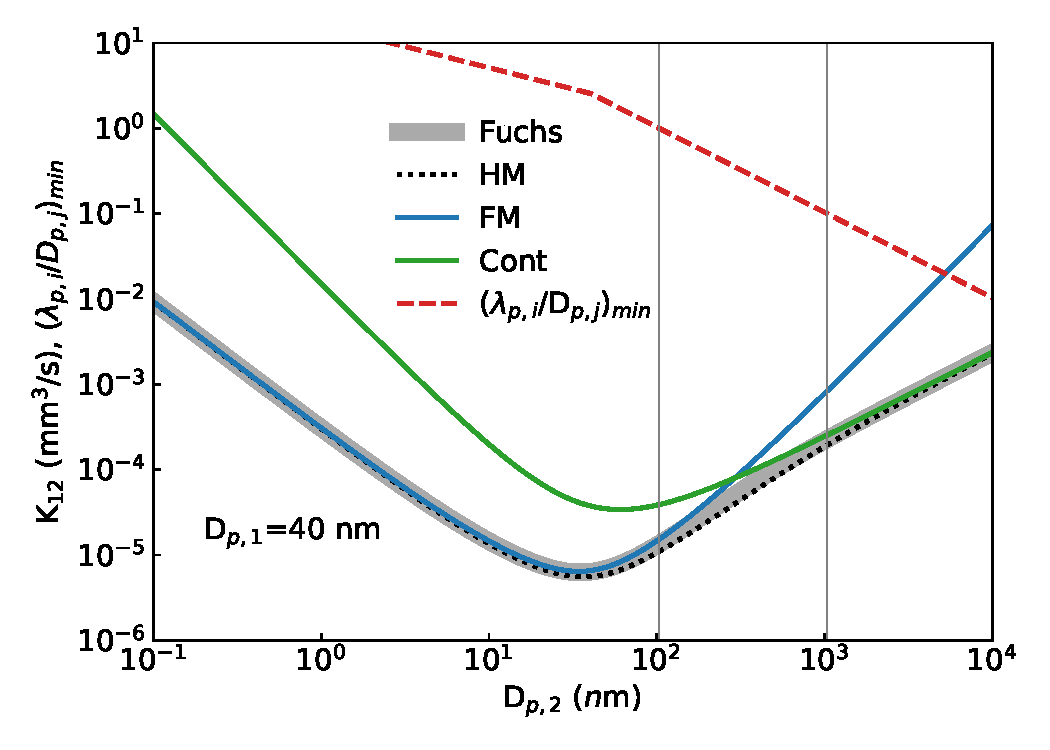
\includegraphics[width=0.8\textwidth]{../figures/coagulation.pdf}
    \end{center}
    \caption{Coagulation coefficient $K_{12}$ for $D_{p,1}$=40 nm.}
    \label{f:coagulation}
\end{figure}
%

%Fuchs proposed a generalized coagulation coefficient of the form $\beta_{12}=2\pi (d_{1}+d_{2})(D_1+D_2)K$, where $K$ is a correction factor that accounts for the kinetic effect of the particle regime~\cite{Fuchs_1964, Seinfeld_2016}.
%In the continuum limit ($Kn \rightarrow 0$), $K=1$ and the Fuchs generalized coagulation coefficient reduces to the continuum regime value, while in the free-molecular limit ($Kn \rightarrow \infty)$, the coagulation coefficient reduces to the free-molecular value.

%Alternatively, the coagulation coefficient in the transition regime can be reasonably approximated by the harmonic mean of the continuum and free-molecular limits~\cite{Kazakov_1998,Frenklach_2002b},
%\begin{equation} \label{e:soot-coag-hm}
%\beta_{12} = \frac{\beta_{\text{C}}\beta_{\text{FM}}}{\beta_{\text{C}} + \beta_{\text{FM}}},
%\end{equation}
%where the subscripts ``C'' and ``FM'' indicate the continuum and free-molecular values of the coagulation coefficient, respectively. Frenklach et~al. reported that using a harmonic mean of the continuum and free-molecular values to represent the transition regime reproduced results given by the Fuchs form of the coagulation coefficient within about 20\%~\cite{Frenklach_2002b}.

SootLib implements four soot coagulation mechanisms derived from the models above. Users can choose the continuum limit (\texttt{CONTINUUM}), the free-molecular limit (\texttt{FM}), the harmonic mean representation of the transition regime (\texttt{HM}), or the Fuchs form of the coagulation coefficient (\texttt{FUCHS}).

%--------------------------------------------------------------------------
\subsection{Particle size distribution and dynamics}
\label{s:PSD_dynamics}

%In addition to chemical reaction, soot particles also undergo non-chemical changes, typically in the form of coagulation, aggregation, and their inverse processes. Instead of treating each possible combination of carbon atoms as its own chemical species, we describe the collection of soot particles as a whole with a particle size distribution (PSD). 
There are two common approaches to modeling aerosol particle size distributions (PSD): sectional and moment methods. Sectional methods divide the domain of particle sizes into discrete ranges based on, e.g., size or mass, while moment methods use the statistical moments of the soot PSD to describe the distribution. In both cases, transport equations defined by the soot variables (sections or moments) interact with the soot chemistry mechanisms to represent the soot evolution during a simulation. Table~\ref{t:psd_models} summarizes the PSD treatments implemented in SootLib.
%
\begin{table}
    \caption{Summary of soot particle size distribution models implemented in SootLib.}
    \label{t:psd_models}
    \centering
    \resizebox{\textwidth}{!}{
        \begin{tabular}{l l l}
            \toprule
            PSD model                                    & Model ID & \# Moments   \\
            \midrule
            Monodisperse~\cite{Lignell_2008b}     & \texttt{MONO}  & 2      \\
            Lognormal~\cite{Lignell_2008b}        & \texttt{LOGN}  & 3  \\
            Quadrature method of moments~\cite{McGraw_1997,Marchisio_2013} & \texttt{QMOM}  & 2, 4, 6, 8  \\
            Method of moments with interpolative closure~\cite{Frenklach_2002b} & \texttt{MOMIC} & 3\textendash8  \\
            Sectional model~\cite{Lehtinen_2001} & \texttt{SECT} & N/A \\
            \bottomrule
        \end{tabular}
    }
\end{table}
%

\subsubsection{Moment methods}
\label{s:moment-methods}

Moment methods describe the PSD using the statistical moments of the distribution. The $k^{th}$ using a discrete PSD is defined by
%
\begin{equation}
    M_k = \sum_i m_i^kN_i,
\end{equation}
%
where the summation is over all possible sizes, and $m_i$ and $N_i$ are the mass (kg) and number density (\#/m$^3$), of size $i$, respectively. For a continuous distribution $M_k$ is defined as
%
\begin{equation} \label{e:mk}
    M_k = \int_0^\infty mn(m)dm,
\end{equation}
%
where $n(m)$ is the number density per unit mass so that $n(m)dm$ is the number of particles per volume between sizes $m$ and $m+dm$.
%where the $k^{th}$ mass moment of the discrete soot PSD is defined by
%\begin{equation} \label{e:moments}
%M_k = \sum_{i=1}^{\infty} m_i^k N_i,
%\end{equation}
%where $m$ is the mass and $N$ is the number density of a given soot particle of size $i$.
In most practical applications, only a small number of moments (2--8) is required to describe the full PSD so that moment methods are computationally more efficient than sectional methods. 

While moments are defined in terms of the PSD, that PSD is unknown and moment source terms must be written directly in terms of the moments, resulting in a closure problem. The closure approach used gives rise to different versions of the method of moments (MOM). For example a transport equation (unsteady in physical space) for soot number density with transport operator $\Gamma$ may be written
as
%
\begin{equation}
    \Gamma(n(m)) = \dot{N} + \dot{G} + \dot{C},
\end{equation}
%
where $\dot{N}$, $\dot{G}$, and $\dot{C}$ are source terms for nucleation, net growth, and coagulation, respectively, which are functions of $n(m)$. The transport equation for $M_k$ is 
%
\begin{equation}
    \Gamma(M_k) = \underbrace{\int_0^\infty m^k\dot{N}dm}_{\dot{N}_k} + 
    \underbrace{\int_0^\infty m^k\dot{G}dm}_{\dot{G}_k}+ 
    \underbrace{\int_0^\infty m^k\dot{C}dm}_{\dot{C}_k}.
\end{equation}
%
Consider the net growth term; it is given by $\dot{G} = -\prtl{ }{m}(v_gn)$, where $v_g=k_s\pi(6/\pi\rho_s)^{2/3}m^{2/3}$ is the growth velocity in the mass coordinate, $k_s$ is the chemical growth rate per unit area, and $\rho_s$ is the soot density. Integrating by parts gives $\dot{G}_k=k\int_0^\infty v_gm^{k-1}n(m)dm$, and insertion of $v_g$ and using the moment definition gives
%
\begin{equation}
    \dot{G}_k = k_s\pi\left(\frac{6}{\pi \rho_s}\right)^{2/3}kM_{k-1/3}.
\end{equation}
%
Transporting integer $k$ moments requires closure of fractional moments $M_{k-1/3}$. Other source terms require similar closures (not shown).

The monodispersed model (\texttt{MONO}) assumes $n(m)=\delta(m-\bar{m})$, where $\bar{m}=M_1/M_0$ and only $M_0$ (the total number of all particles per volume) and $M_1$ (the mass density of soot particles) are considered. The \texttt{LOGN} model assumes the PSD is lognormal~\cite{Pratsinis_1988}. In this case, fractional moments are given in terms of the first three integer moments $M_0$, $M_1$, and $M_2$~\cite{Lignell_2008b}
%
\begin{equation}
    M_k = M_0^{1-\frac{3}{2}k+\frac{1}{2}k^2} M_1^{2k-k^2} M_2^{\frac{1}{2}k^2-\frac{1}{2}k}.
\end{equation}
%
The quadrature method of moments (\texttt{QMOM}) assumes the PSD is given by
%
\begin{equation} \label{e:nqmom}
    n(m) = \sum_{\alpha=1}^{N_e}w_\alpha\delta(m-m_\alpha),
\end{equation}
%
where $N_e$ is the number of particle \emph{environments}, (half the number of moments considered), and $w_\alpha$ and $m_\alpha$ are the number density and particle mass in environment $\alpha$, which can be solved algebraically~\cite{Wheeler_1974, Marchisio_2013} using Eqs.~(\ref{e:mk},\ref{e:nqmom}). Given the assumed forms for $n(m)$ in these three PSD models, the integrals in the moment source terms can be directly evaluated.

%Moment transport equations take the form
%\begin{equation}
%    \label{e:momTransEq}
%    \frac{\partial M_k}{\partial t} + \frac{\partial v_k M_k}{\partial x_k} = -\frac{\partial M_k v_T}{\partial x_k} + S_k,
%\end{equation}
%where the velocity $v_k$ and the thermophoretic diffusion velocity $v_T$ are assumed to be independent of particle size.\footnote{This is a reasonable assumption for small soot particles transported mainly by convection and thermophoresis.} $S_k$ represents the moment source term, which is comprised of the sum of individual moment source terms for the soot chemistry steps, usually one each for nucleation, surface growth, oxidation, and coagulation.

%While moment equations are exact, their source terms are unclosed---typically requiring fractional moment values---and closure models are required to calculate them. Moment methods differ amongst themselves primarily in their approach to source term closure.

%SootLib includes four moment models for calculating the source terms of the moment transport equations, summarized in~\ref{t:psd_models}. Two of the models---\texttt{MONO} and \texttt{LOGN}---assume a particular shape for the soot PSD in order to close the source terms. The two remaining models---\texttt{QMOM} and \texttt{MOMIC}---do not assume a shape for the PSD; instead, they obtain values for the unclosed fractional moments via numerical quadrature and interpolation, respectively.

%SootLib's simplest moment closure model is the assumed monodisperse size distribution (\texttt{MONO}), which requires only the first two moments of the soot PSD, which correspond to the overall particle number density and mass density of soot particles. Because it describes the PSD with only two moments, moment source terms can be closed with relatively simple analytic expressions~\cite{Lignell_2008b}, making it a popular starting point for soot PSD modeling.
%Its accuracy may be sufficient for simple flame configurations that produce relatively small soot particles in relatively small quantities.

%The assumed lognormal distribution model (\texttt{LOGN}) builds on the simplicity of the \texttt{MONO} model by adding a third mass moment and assuming that the soot PSD can be described by a lognormal distribution rather than a monodisperse distribution~\cite{Lignell_2008b}. Whole-order moments are transported via the moment transport equations, and fractional moments can be calculated from the whole-order moments with an analytic expression.
%as
%\begin{equation}
%    M_k = M_0^{1-\frac{3}{2}k+\frac{1}{2}k^2} M_1^{2k-k^2} M_2^{\frac{1}{2}k^2-\frac{1}{2}k}.
%\end{equation}
%As with the \texttt{MONO} model, the \texttt{LOGN} model is straightforward and computationally efficient, but it also increases the potential for accuracy. Experimental studies show that the soot PSD is generally bimodal, which can be reasonably approximated by the combination of a lognormal distribution and a power law function~\cite{Zhao_2003,Zhao_2003b,Wang_2009,Wang_2011,Gu_2016}. While the lognormal part of this representation represents the bulk of the soot population, neglecting the power law portion can still decrease accuracy when modeling a soot PSD with an assumed lognormal distribution.

%Higher accuracy can be obtained by avoiding assuming the shape of the soot PSD, but this requires an alternate approach to closing the moment source terms. The quadrature method of moments (QMOM) does this by applying numerical quadrature to the unknown PSD~\cite{McGraw_1997}. SootLib applies the Wheeler algorithm for moment inversion to calculate the weights and abscissas of the unknown soot PSD~\cite{Marchisio_2013,Wheeler_1974}.
%For a set of $n$ whole-order moments, resulting in $n/2$ weights $w_i$ and abscissas $a_i$ from the inversion algorithm, fractional moments can be calculated with
%\begin{equation} \label{e:soot-models-psd-mk}
%M_k = \sum_{i=1}^{n/2} w_i a_i^k.
%\end{equation}
%Avoiding specifying a shape for the soot PSD significantly increases the accuracy of the model, particularly when the distribution increases in complexity, and while this does increase the computational resources required, efficient inversion algorithms and careful implementation can reduce it to acceptable levels.

The method of moments with interpolative closure (MOMIC) avoids specifying the shape of the soot PSD and closes the moment source terms by interpolating between whole order moments to calculate fractional moments. 
%This potentially increases its numerical efficiency over quadrature methods while retaining similar levels of accuracy. 
SootLib implements MOMIC as described by Frenklach~\cite{Frenklach_2002b,Frenklach_1987}
using polynomial interpolation between logarithms of the whole-order moments. The form of the free molecular coagulation coefficient requires special treatment in both MOMIC and the lognormal closure approaches as described in the source documentation and literature.


%As noted above, experimental studies show that the soot PSD is generally bimodal and may be reasonably approximated by the combination of a lognormal distribution and a power law function~\cite{Zhao_2003,Zhao_2003b,Wang_2009,Wang_2011,Gu_2016}. It is straightforward to generate an expression for an arbitrary moment based on the distribution parameters, but a nonlinear solver is required to calculate distribution parameters from a given moment set, potentially increasing the time and computational cost of the calculation~\cite{Lignell_2008b}. Additionally, such a distribution still assumes a form for the soot PSD---albeit a more complex one---which restricts its evolution. Under these conditions, it is reasonable to choose methods like QMOM and MOMIC that do not assume a shape for the soot PSD; they can still produce the desired bimodal distribution given a sufficient moment set but have neither the restrictions nor the additional computational overhead of an assumed bimodal distribution. Assumed bimodal distribution models are not typical for these reasons, and, as such, SootLib does not include any models of this type.

\subsubsection{Sectional model}
\label{s:sectional}

Sectional models represent the PSD directly---rather than through its statistical moments---using the particle number density in a defined set of sections (or \emph{bins}) that represent the discretized domain. In the \texttt{SECT} model, the desired number of bins are spaced geometrically by a variable by default factor of two.
%Rather than transporting moments, SootLib's sectional model---\texttt{SECT}---transports the particle number density in each section, or bin, on the domain.
%\begin{equation} \label{e:psd-sectional}
%\frac{\partial N_k}{\partial t} + \frac{\partial v_k N_k}{\partial x_k} = -\frac{\partial N_k v_T}{\partial x_k} + S_k,
%\end{equation}
%where $N_k$ represents the number density of soot particles in the $k^{th}$ size section. As in~\eqref{e:momTransEq}, the velocity $v_k$ and the thermophoretic diffusion velocity $v_T$ are independent of particle size. Here, $S_k$ is a number density source term rather than a moment source term, but it still represents the sum of the individual soot chemistry source terms---nucleation, surface growth, oxidation, and coagulation---in the $k^{th}$ size section.

Sectional models do not require the same type of closure that moment methods do, but coagulation between particles usually results in particles with sizes between given section sizes. Since the particles can only reside in the given sections, the intermediate size is modeled by assigning a number of particles to each of the two neighboring sections so that total mass and number are conserved~\cite{Lehtinen_2001}. Any particles formed that are larger than the last section are placed in that section in an amount to conserve mass. Growth and oxidation are represented by a velocity in the size coordinate. SootLib uses an upwind method to maintain stability, but higher order monotone schemes for conservation laws (e.g., flux limiters) can implemented.
%they do require treatment for cases in which coagulation creates particles that do not fit neatly in one of the predefined size bins. 
%a size-splitting operator is included in the discrete coagulation equation~\cite{Lehtinen_2001}, ensuring that particles are divided in the correct proportions to conserve mass and particle number in cases where a collision produces a particle that does not fit neatly into one size class.

The advantage of the sectional model over the MOM is that it gives a direct representation of the PSD, and is potentially more accurate if sufficient resolution is included. The disadvantage is the many more sections (and hence soot variables) are required than is typical in the MOM. In both cases, $M_0$ and $M_1$ are the primary variables of interest, with $M_1/\rho_s$ being the soot volume fraction that is most commonly measured experimentally.

%The accuracy of any sectional model depends on the resolution of its domain; the more sections that are defined, the closer the approximation gets to describing the true soot PSD, but the higher the computational cost becomes. A sectional model might require hundreds or even thousands of sections, each with its own transport equation, to achieve the same level of accuracy achieved by only a handful of moment transport equations, which represents a significant investment of computational cost and time. It can be advantageous, however, because it makes no assumptions about the shape, size, or behavior of the PSD, making sectional methods valuable tools for investigating fundamental physical phenomena and validating models.

\subsection{Model combinations and limitations}
\label{s:limitations}

SootLib is designed to be semi-modular in that the various soot chemistry mechanisms can be substituted and exchanged, providing users with increased flexibility. It must be noted, however, that not all model combinations will produce physically meaningful results, either due to a model's design or its author's intent. The following notes indicate some limitations to be aware of when choosing model combinations.

SootLib computes soot variable source terms using a specified gas and soot variable state, usually as part of separate reacting flow simulation tool, such as for a premixed flame, in which energy and gas composition profiles are solved. In this case, the gas-phase chemistry mechanism should include the species required by the chosen soot chemistry mechanisms. However, SootLib is fully independent of such a gas mechanism, and the gas composition vector SootLib uses is whatever the user provides.  
%When using SootLib for combustion CFD, the gas-phase chemistry mechanism must include the gas species required by the chosen soot chemistry mechanisms. 
%For instance, a one-step global ethylene mechanism for gas chemistry will generate zero-value source terms for the soot nucleation and growth because it does not include the acetylene or gaseous PAH required by SootLib's nucleation mechanisms.
%SootLib does not explicitly warn users when such situations occur, as there may be cases in which a user finds it advantageous or instructive to exclude or explicitly set a gas species concentration. Therefore, users must take care to choose soot chemistry mechanisms that are appropriate to their use case.
%% DOL: I don't want to go into the PAH nucleation too much here, since it is not too general yet.
%In particular, note that the \texttt{PAH} nucleation mechanism uses the concentrations of a small subset of gaseous PAH molecules; if none of the relevant PAH species is present in the gas mechanism, no soot nucleation will occur. Refer to the SootLib package documentation for more details.

The following points apply to model specification:
\begin{itemize}
\item The \texttt{LL} model is included with SootLib as a point of reference because it is common in combustion simulation studies. This model was developed from experimental ethylene jet flames, and its accuracy and applicability are generally limited to conditions similar to those under which it was developed.
%DOL: this is implied in the code/code options: \item The Leung and Lindstedt model as presented in~\cite{Leung_1991} includes a coagulation mechanism that is a modified free-molecular regime model, so it is not explicitly implemented in SootLib. Refer to the package documentation for instructions on obtaining the equivalent of Leung and Lindstedt's coagulation results.
%    Instead, users can obtain the equivalent of Leung and Linstedt's coagulation results by choosing \texttt{FM} coagulation and modifying the \texttt{FM\_multiplier} variable by calling the auxiliary \texttt{set\_FM\_multiplier} function with the argument \texttt{9/2/eps\_c}.
\item The \texttt{HACA} surface growth and oxidation mechanisms should not be used separately. The code will give a warning otherwise. %if the user attempts to combine HACA surface growth with non-HACA oxidation or vice versa.
\item The \texttt{PAH} nucleation mechanism also results in PAH condensation~\cite{Blanquart_2009c}; these may be separated in a future release.
\item The \texttt{PAH} nucleation mechanism assumes that the self-collision of PAH molecules occurs in the free-molecular regime independent of the coagulation model specified by the user. %, which cannot be overridden by the user's coagulation mechanism selection. Dimer self-collisions and PAH--soot condensation collisions do not explicitly specify a coagulation regime, so their calculations do depend on which coagulation mechanism the user selects.
\end{itemize}
%

%As discussed later in Section~\ref{s:soot-examples-compcost}, choosing a soot PSD model for combustion simulations often involves a balance between accuracy and computational cost. While the 2-moment \texttt{MONO} and 3-moment \texttt{LOGN} models are significantly faster than \texttt{QMOM} and \texttt{MOMIC}, they are relatively inflexible.
%%That simplicity, however, can be convenient and appropriate for certain applications, such as simulating flames in which soot occurs in relatively small amounts.
%Methods like QMOM and MOMIC that do not make assumptions about the underlying shape of the soot PSD are advantageous because they allow the soot distribution to evolve naturally, and the number of moments can be increased to meet accuracy requirements. The more moments that are used to describe the distribution, the more accurately that moment set represents the underlying distribution, but increasing the number of moments can also significantly increase the computational cost of the model.

Regarding the PSD model chosen, \texttt{QMOM} requires an even number of moments. The \texttt{MONO} and \texttt{QMOM} with two moments are verified to give identical results, but the \texttt{MONO} is simpler and has somewhat less computational overhead. Both \texttt{MOMIC} and \texttt{QMOM} are limited to eight moments, but no more than six should generally be needed.

%Consider the following points when choosing a soot PSD model for simulations:
%\begin{itemize}
%    \item Due to the nature of numerical quadrature, \texttt{QMOM} is limited to even-numbered moment sets ($N=2,4,6,8\ldots$).
%%    \item The \texttt{QMOM} model can become unstable when used with more than six moments. If more moments are required, consider using \texttt{MOMIC}, which can accommodate up to eight moments, including odd-numbered moment sets.
%    \item A 2-moment QMOM model is functionally equivalent to a monodisperse distribution (MONO), but has some additional overhead associated with its implementation. Given a choice, the \texttt{MONO} model is generally preferable to a 2-moment \texttt{QMOM} model.
%%    \item For general-purpose soot modeling within combustion simulations using moment methods for the soot PSD, four moments is a good starting point and is generally sufficient to describe a soot PSD for simple gaseous fuels. For more complex fuels or cases requiring higher accuracy, more moments may be required.
%\end{itemize}

%At present, SootLib does not include any models that account for the agglomeration of soot particles into large fractal aggregate structures, which require at least two variables to accurately represent both the size and shape of a particle. While bivariate PSD models for soot aggregation exist~\cite{Wright_2001,Mueller_2009,Blanquart_2009c}, they tend to be computationally expensive and difficult to implement. SootLib does not currently implement any multivariate models, but its framework can potentially accommodate them, making it well-positioned to support this area of active research and development.

%While it is well known that soot particles tend to form fractal aggregates, simulation of the fractal structure of soot particles is still a relatively young area of research~\cite{Patterson_2007}. Unlike spherical particles, fractal aggregate structures require at least two variables to accurately represent both the size and shape of a particle, and while bivariate PSD models for soot aggregation exist~\cite{Wright_2001,Mueller_2009,Blanquart_2009c}, they tend to be computationally expensive and difficult to implement. While SootLib does not currently implement any multivariate models, its framework can potentially accommodate them, making it well-positioned to support this area of active research and development.

%%%%%%%%%%%%%%%%%%%%%%%%%%%%%%%%%%%%%%%%%%%%%%%%%%%%%%%%%%%%%%%%%%%%%%%%%%%

\section{Software description}
\label{s:architecture}

SootLib is an object-oriented C++ library intended for use in reacting flow simulations including CFD.
Upon download, the SootLib package contains four directories: 
%
\begin{itemize}
    \item \texttt{src} contains the SootLib source code; 
    \item \texttt{examples} contains usage example codes; 
    \item \texttt{tests} contains SootLib's optional testing suite, driven by Catch2; and 
    \item \texttt{docs} contains the files optionally used to generate code documentation with Doxygen.
\end{itemize}
%
SootLib installation is automated by CMake, and project options can be changed by editing the top-level \texttt{CMakeLists.txt} file or by editing the \texttt{CMakeCache.txt} file. Refer to the package documentation for detailed compilation and installation instructions, including a full list of CMake options.
%To build and install the library with the default settings, the user must create and navigate into the \texttt{build} directory and execute the following commands:
%\begin{enumerate}
%    \item \texttt{cmake ..}
%    \item \texttt{make}
%    \item \texttt{make install}
%\end{enumerate}

Successful installation will generate an \texttt{include/sootlib} directory that contains SootLib's header files and a \texttt{lib} directory that contains the library file, \texttt{libsootModel.a} and SootLib's relocatable CMake package, \texttt{sootlib.cmake}.
%Successful installation will generate the following additional directories and files:
%\begin{itemize}
%    \item[\faFolderO] \texttt{include}
%    \begin{itemize}
%        \item[\faFolderO] \texttt{sootlib}
%        \begin{itemize}
%            \item[\faFileTextO] \texttt{constants.h}
%            \item[\faFileTextO] \texttt{sootModel.h}
%            \item[\faFileTextO] \texttt{state.h}
%        \end{itemize}
%    \end{itemize}
%    \item[\faFolderO] \texttt{lib}
%    \begin{itemize}
%        \item[\faFolderO] \texttt{cmake}
%        \begin{itemize}
%            \item[\faFolderO] \texttt{sootlib}
%            \begin{itemize}
%                \item[\faFileCodeO] \texttt{sootlib.cmake}
%            \end{itemize}
%        \end{itemize}
%        \item[\faFileCodeO] \texttt{libsootModel.a}
%    \end{itemize}
%\end{itemize}
To use SootLib in C++ code, include the installed header file \texttt{sootHeaders.h} and link the \texttt{libsootModel.a} library file. Alternately, SootLib can also be used as part of larger CMake projects via \texttt{sootlib.cmake} or CMake's FetchContent module.

The SootLib library consists primarily of two object classes through which the user interacts with the library---\texttt{state} and \texttt{sootModel}---both of which are contained within the \texttt{soot} namespace. The \texttt{state} object holds user-supplied details about the current thermodynamic state: temperature, pressure, density, viscosity, gas species mass fractions, and soot variable quantities (a vector of moments or section number densities). The \texttt{sootModel} object contains information about the selected models and performs the calculations that generate source terms for the sectional or moment transport equations. The \texttt{sootModel} is constructed by setting the number of soot variables and the desired nucleation, growth, oxidation, and coagulation models. Those models can be set either through an enumeration variable or by creating the respective model objects.
%In the context of a traditional CFD simulation, the \texttt{state} object would be updated via the \texttt{setState} function at each time step and/or grid point and followed by a call to \texttt{calcSourceTerms}, whereas the \texttt{sootModel} parameters only need to be specified once when the object is created.
The resulting soot and gas species source terms are accessed via the \texttt{sootModel} object's \texttt{sourceTerms} struct called \texttt{sources}. Refer to the package documentation and examples for further details on using the SootLib library.

SootLib's two major functionalities are:
\begin{itemize}
    \item Calculates source terms for the soot transport equations given thermodynamic state details and chemistry mechanisms chosen by the user; and
    \item Calculates mass source terms for gaseous chemical species affected by soot chemistry.
\end{itemize}

%%%%%%%%%%%%%%%%%%%%%%%%%%%%%%%%%%%%%%%%%%%%%%%%%%%%%%%%%%%%%%%%%%%%%%%%%%%

\section{Examples}
\label{s:examples}

%We refer to the literature and the references indicated in Section~\ref{s:models} for the validation of individual models included in Sootlib.

%Each of SootLib's models was implemented and validated according to the mathematics presented in the literature.

Two examples are provided with SootLib. 
\texttt{simple\textunderscore example.cc} is provided as a basic, standalone example of soot model setup, source term calculation, and source term retrieval to illustrate use of the SootLib library. This format has limited functionality, but can be useful for directly comparing various models' source term calculations. 
%The results of running this example may or may not be physically significant, depending on its inputs; 
It is primarily intended as an illustration of how to set up and interact with the library. The second example is a burner-stabilized premixed flame.

\subsection{Premixed burner example}
\label{s:soot-examples-premixed}

By way of demonstration, we coupled SootLib with the one-dimensional burner stabilized premixed flame code in Cantera~\cite{Cantera}. We consider ISF laminar premixed flame 2~\cite{ISF4-P2}, an ethylene--air fuel mixture with an equivalence ratio $\phi=2.34$ flowing at a velocity of \qty{6.73}{\cm/\s}---and compare simulation results to the three sets of exper:wwwimental data provided in this configuration~\cite{Xu_1997,Menon_2007}.

The simulation case used the GRI 3.0 gas chemistry mechanism~\cite{Smith_2002}. Soot chemistry is described with the \texttt{LIN} nucleation mechanism~\cite{Lindstedt_2005}, \texttt{LIN} surface growth~\cite{Lindstedt_1994}, \texttt{LL} oxidation~\cite{Leung_1991}, free-molecular coagulation~\cite{Seinfeld_2016}, and the monodisperse PSD model (\texttt{MONO}).
%We also performed a simple comparison in this configuration by running two more simulations in which only the coagulation mechanism was altered.

Figure~\ref{f:soot-premix} shows the simulation results for soot volume fraction as a function of height above the burner surface along with experimental values. 
The simulation results agree well with the experimental data though there is significant variation in the experimental soot volume fraction. The soot model used kinetic data fitted to experiments of diffusion flames and assumed free molecular coagulation. The soot volume fraction is about an order of magnitude higher at high burner heights if the harmonic mean or Fuchs coagulation models are used instead, which results in more particles and more surface area for growth.
%snbut fall below the measurements in the third experimental data set.\footnote{The third data set was obtained by a different research group than the first and second data sets. Deviations may be attributable to differences in the experimental apparatus or external conditions, though the precise cause is unclear.}
%%While we might anticipate that a transition regime mechanism like \texttt{FUCHS} or \texttt{HM} would predict soot volume fractions more accurately, we observe the opposite in this case.
%The \texttt{LL} and \texttt{LIN} mechanisms were developed under the assumption of free-molecular coagulation; because they are empirical rate expressions, it makes sense that the \texttt{FM} mechanism would produce better agreement than the transition regime mechanisms.
%
\begin{figure}
    \begin{center}
        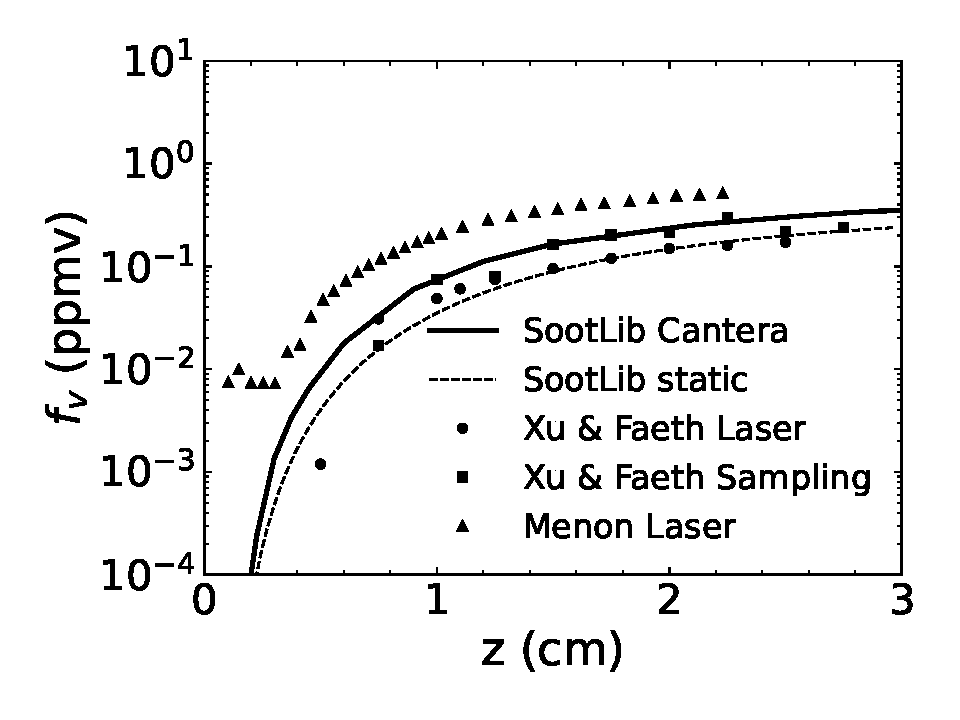
\includegraphics[width=0.8\textwidth]{../figures/premixed/burner.pdf}
    \end{center}
    \caption{Premixed burner flame comparing simulation to experimental data.}
    \label{f:soot-premix}
\end{figure}
%

SootLib provides a second example \texttt{burner\textunderscore flame.cc} that integrates soot variables using static temperature, velocity, density, viscosity, and gas mass fraction profiles from the Cantera simulation discussed above. This gives a relevant example while allowing independence from third-party simulation codes. The soot equations solved are $dM_k/dz = \dot{M}_k/\rho v$, where $\rho$ and $v$ are the gas density and velocity profiles. Differences between the two simulations are due to neglecting diffusion effects and gas-soot coupling in the static simulation.

Figure~\ref{f:sectional} shows the \texttt{burner\textunderscore flame.cc} example output using the sectional model with 40 soot sizes. The size distribution is shown at eight burner heights showing its evolution from the power-law nucleation mode at early times to including the lognormally-distributed coagulation mode at later times.
%
\begin{figure}
    \begin{center}
        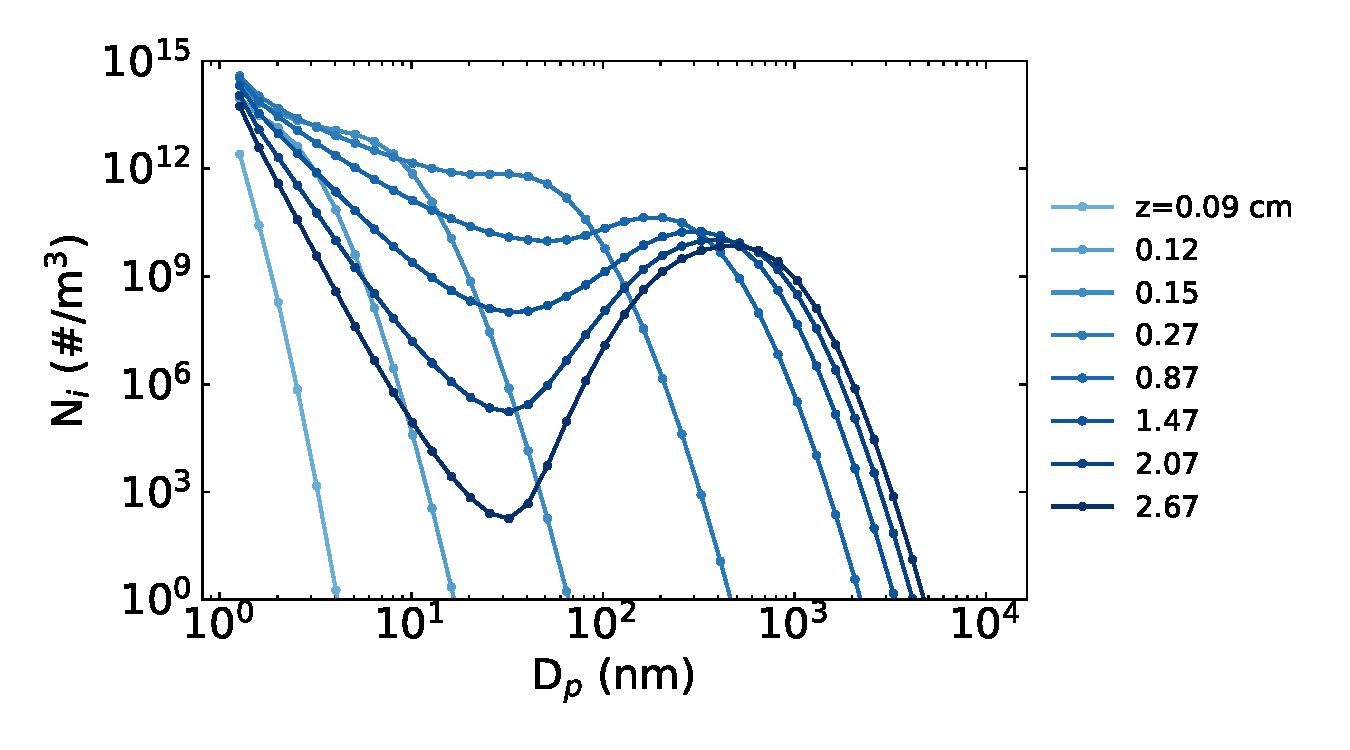
\includegraphics[width=0.8\textwidth]{../figures/premixed/sectional/sectional.pdf}
    \end{center}
    \caption{Premixed burner flame using the sectional model showing the evolution of the PSD.}
    \label{f:sectional}
\end{figure}
%

Computational cost comparisons of the various models have been performed. These results are presented in the source documentation files (Doxygen).

%%%%%%%%%%%%%%%%%%%%%%%%%%%%%%%%%%%%%%%%%%%%%%%%%%%%%%%%%%%%%%%%%%%%%%%%%%%

%\subsection{Computational cost}
%\label{s:soot-examples-compcost}
%
%We also compared the computational cost of the implemented soot models, represented by the time required for one thousand evaluations of the \texttt{calcSourceTerms} function averaged over one hundred trials.\footnote{Comparisons were performed using a 3.5~\si{GHz} Intel i5-7400 CPU with 8~\si{GB} of available RAM via Windows Subsystem for Linux (WSL).} The base \texttt{sootModel} object used for comparisons was initialized with \texttt{LL} chemistry and a 4-moment \texttt{QMOM} PSD treatment, and the \texttt{state} object represents a stoichiometric ethylene--air mixture, initially at 1~\si{atm} and 298~\si{K}, equilibrated by Cantera~\cite{Cantera} at constant pressure and enthalpy.
%
%Figure~\ref{f:cost_chem} summarizes the relative cost of soot chemistry models, where only the model in question differs from the base \texttt{sootModel} object. Results are normalized by the runtime of the base \texttt{sootModel} configuration, which required an average of 0.3156~\si{s}.
%Even though there are differences in the mean computational time for soot chemistry models, they may or may not represent a significant addition to the computational cost of a combustion simulation as a whole.
%%
%\begin{figure}
%    \begin{center}
%        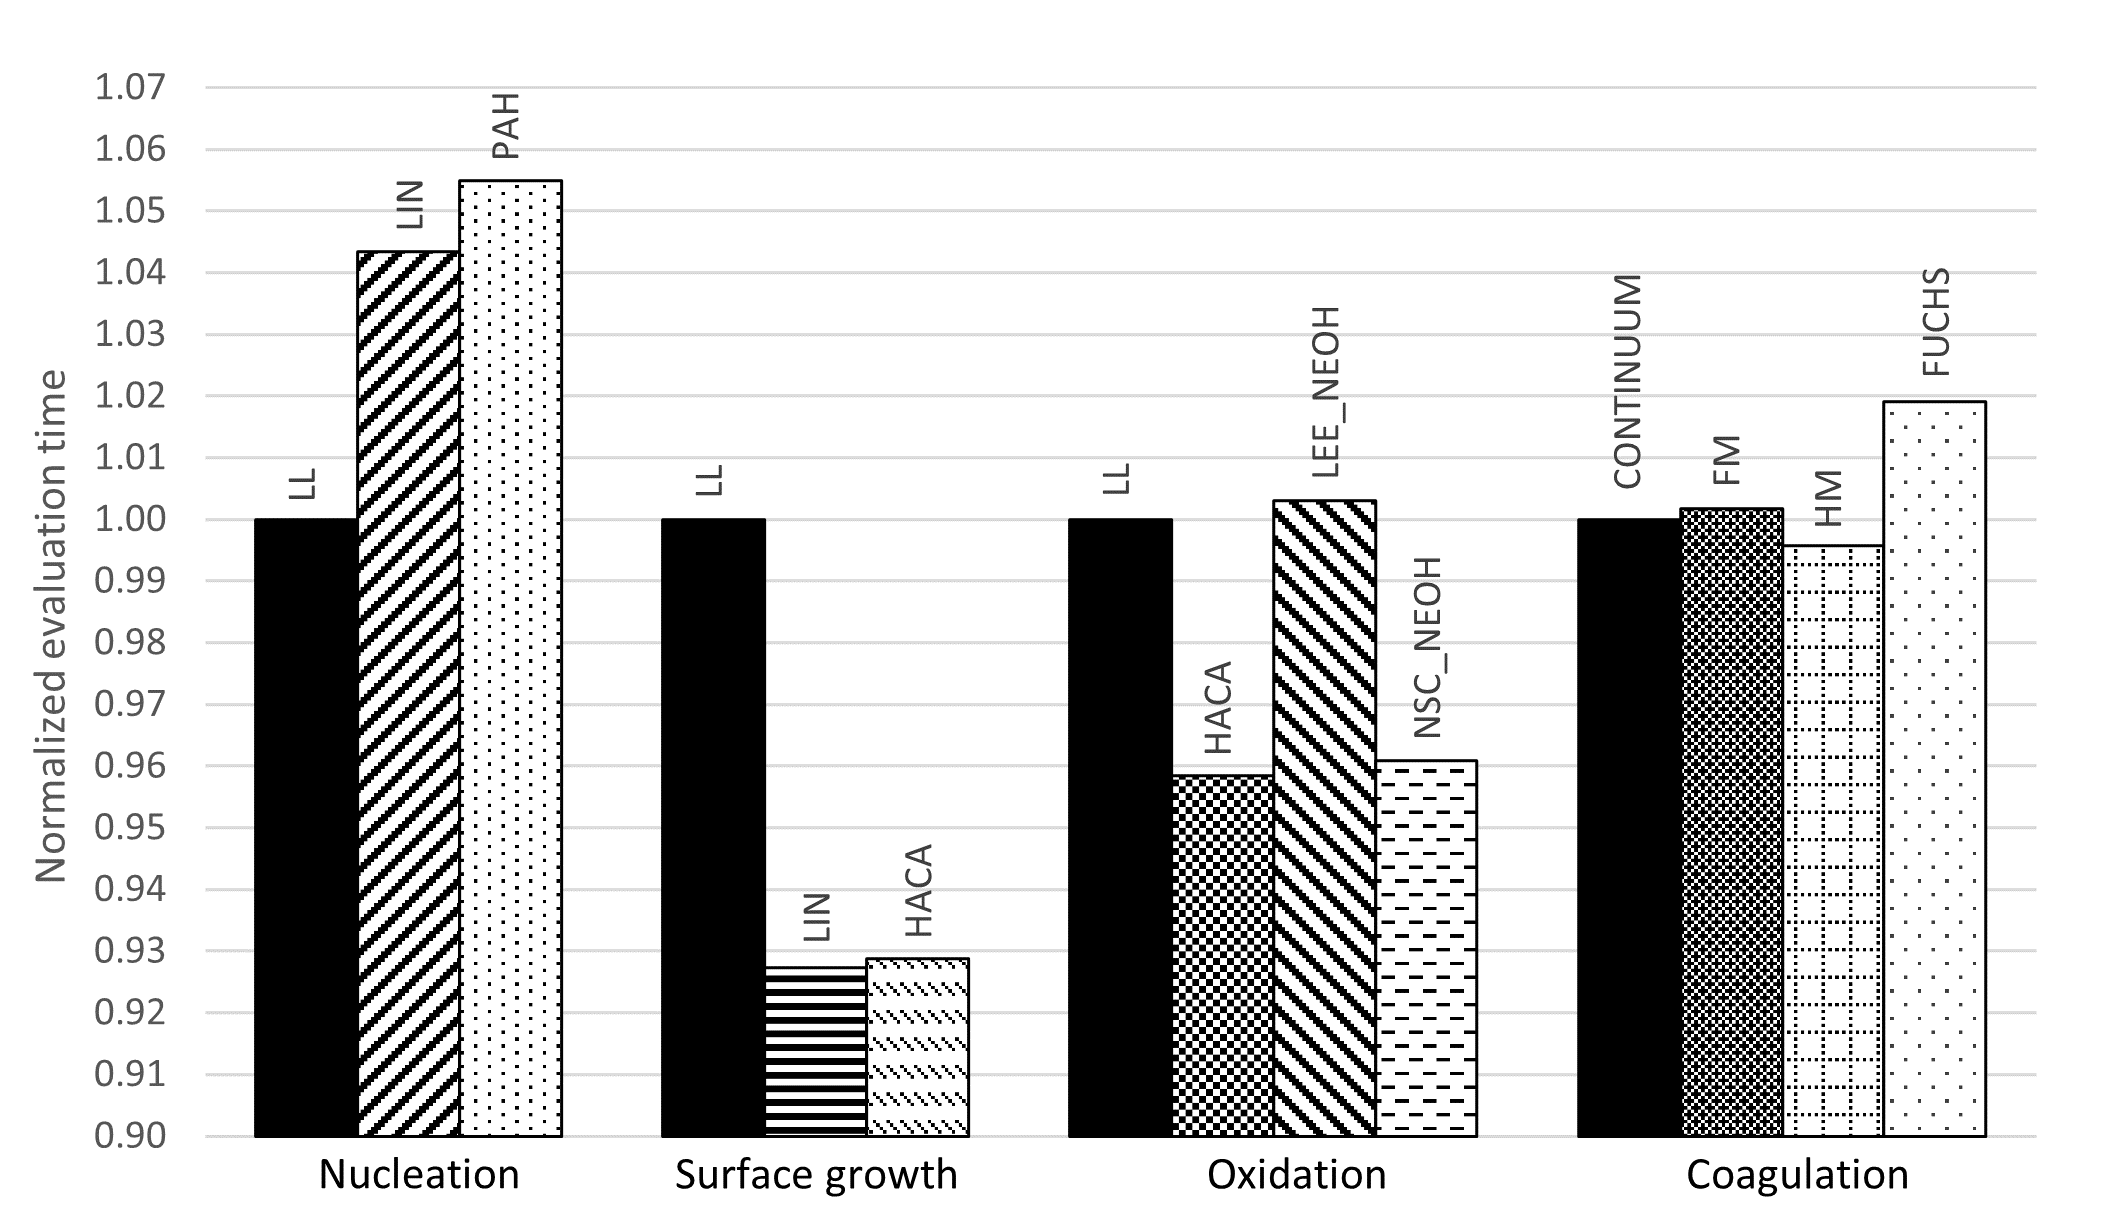
\includegraphics[width=\textwidth]{../figures/comp_cost_chem}
%    \end{center}
%    \caption{Comparison of the computational cost of the soot chemistry models implemented in SootLib. Computational times are normalized by the cost of the base \texttt{sootModel} configuration, which consists of \texttt{LL} chemistry and a 4-moment \texttt{QMOM} PSD treatment.}
%    \label{f:cost_chem}
%\end{figure}
%%
%
%Figure~\ref{f:cost_PSD} compares the relative computational cost of SootLib's implemented PSD models using the same criteria as the chemistry comparison, where only the PSD model or the number of moments used differs from the base \texttt{sootModel} configuration. Results are normalized by the runtime of the 2-moment \texttt{MONO} configuration, which required an average of 0.2961~\si{s}.
%The \texttt{MOMIC} configurations are presented on a separate plot to highlight the difference in scale compared to the \texttt{MONO}, \texttt{LOGN}, and \texttt{QMOM} models.
%\begin{figure}
%    \begin{minipage}{0.5\textwidth}
%        \centering
%        (a) \\ 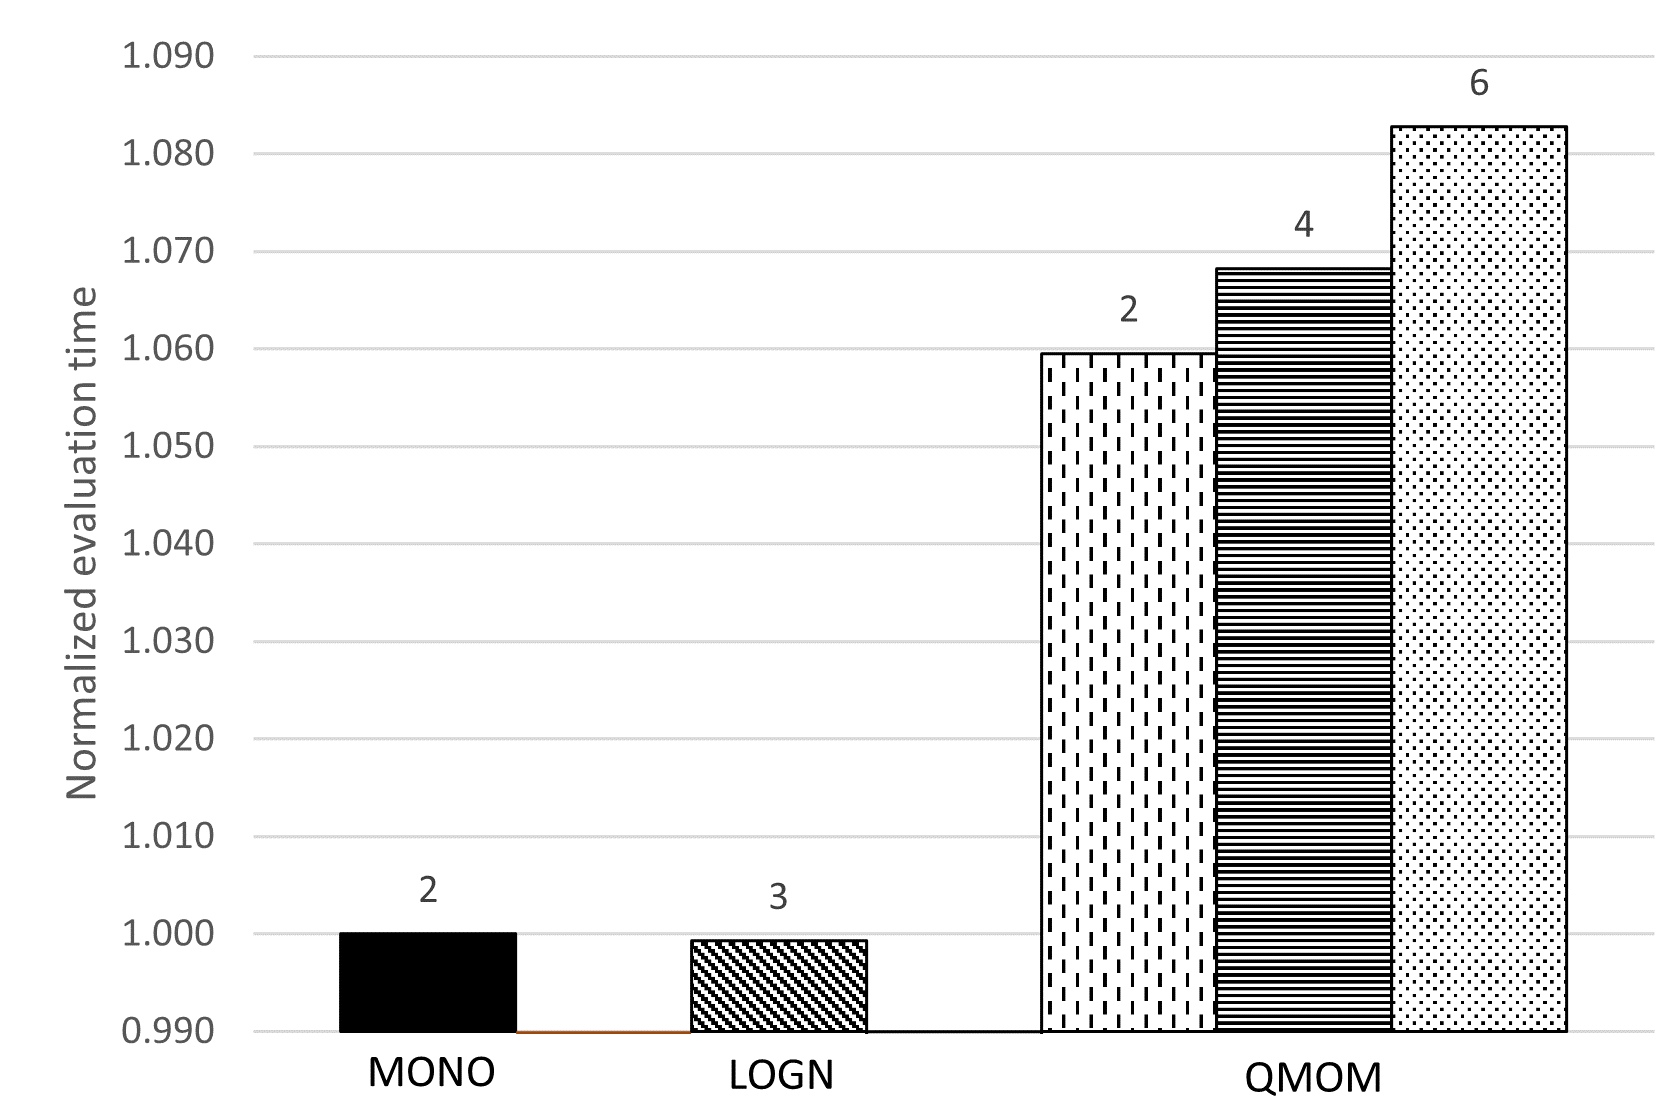
\includegraphics[width=0.98\textwidth]{../figures/comp_cost_PSDa}
%    \end{minipage}
%    \begin{minipage}{0.5\textwidth}
%        \centering
%        (b) \\ 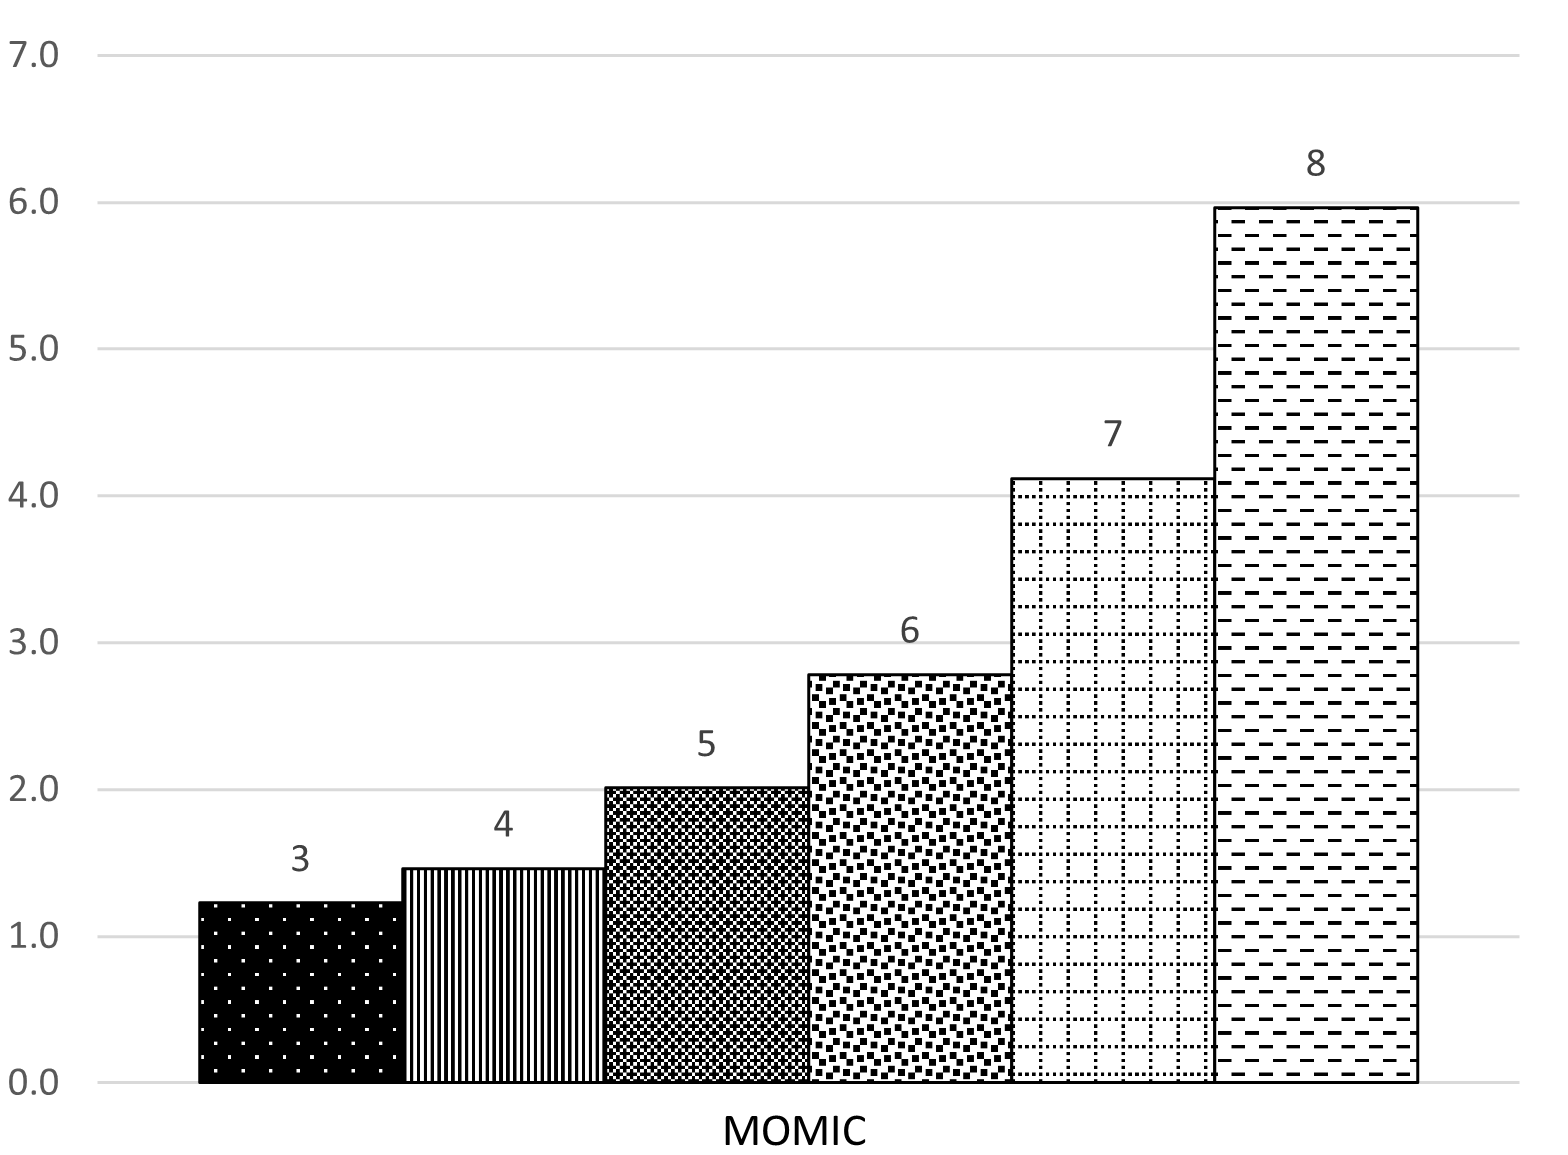
\includegraphics[width=0.98\textwidth]{../figures/comp_cost_PSDb}
%    \end{minipage}
%    \caption{Comparison of the computational cost of the soot PSD models implemented in SootLib, including (a) \texttt{MONO}, \texttt{LOGN}, and \texttt{QMOM} (with 2, 4, and 6 moments) and (b) \texttt{MOMIC} (with 3--8 moments). The number above each bar indicates the number of moments used. Results are normalized by the runtime of the \texttt{MONO} configuration with \texttt{LL} chemistry.}
%    \label{f:cost_PSD}
%\end{figure}
%
%%It is well known that the computational cost of a sectional model depends on the number of sections---and therefore the number of transport equations---defined for the system, so a comparison to that effect is not included here. Additionally, sections interact with one another differently than moments do, so a direct comparison between the sectional model and any of the moment methods would not necessarily be meaningful.
%
%Comparison of Figures~\ref{f:cost_chem} and~\ref{f:cost_PSD} reveals two important points to consider when choosing soot model parameters for combustion simulations. First, the choice of soot chemistry presents much less variation in computational time than the choice of PSD model. That is, choosing a more complex combination of soot chemistry models is unlikely to affect the overall computational cost of a simulation as much as choosing a more complex PSD model would. Second, the choice of PSD treatment and the number of moments to use is non-trivial. As discussed in Section~\ref{s:limitations}, assuming a shape for the soot PSD requires significantly less computational time than more complex methods, but comes at the expense of accuracy and flexibility. Thus, choosing an appropriate soot PSD model often becomes a question of balance between accuracy and computational cost.

%%%%%%%%%%%%%%%%%%%%%%%%%%%%%%%%%%%%%%%%%%%%%%%%%%%%%%%%%%%%%%%%%%%%%%%%%%%

\section{Conclusion}
\label{s:soot-conclusion}

To the authors' best knowledge, there is no existing tool like SootLib, which combines various soot models into one package on a consistent, cross-platform, open-source framework that is not specific to any one CFD code or simulation type. It requires no external dependencies, and it can be used in C++ projects directly or included in larger CMake projects via its exported package or CMake's FetchContent module. Users interact with the SootLib library through a small group of objects and functions that allow them to specify model parameters, set a thermodynamic state and composition for the gas environment, and calculate source terms for moment transport equations.

SootLib is intended to be a convenient tool that provides combustion researchers with more options and more control over simulations involving sooting flames. For researchers who do not specialize in soot but require soot modeling in order to perform accurate simulations, SootLib lowers the barrier to entry on the topic; it requires a minimum of prior knowledge to use, representing a significant time savings to its users. For combustion researchers who do specialize in soot, SootLib's uniform framework and modular design make it a good comparative tool, increasing the potential for useful parametric studies involving soot and decreasing the overhead involved with testing new and existing soot models under a variety of conditions.

SootLib has been implemented into both Cantera~\cite{Cantera} and in the One-Dimensional Turbulence ODT code~\cite{Stephens_2021}. 

%At present, SootLib is being used both independently and as part of the larger development of the ODT code~\cite{Stephens_2021}. When coupled with the RadLib library~\cite{Stephens_2022}, SootLib promises to leverage the low computational cost of the ODT model to perform parametric simulation studies of sooting jet flames that include late-flame soot evolution and soot-flame breakthrough, representing parameter ranges that are typically inaccessible in high-resolution combustion CFD due to excessively high computational cost.


%%%%%%%%%%%%%%%%%%%%%%%%%%%%%%%%%%%%%%%%%%%%%%%%%%%%%%%%%%%%%%%%%%%%%%%%%%%

\section{Conflict of Interest}
%Please select the appropriate text:

%Potential conflict of interest exists:
%We wish to draw the attention of the Editor to the following facts, which may be considered as potential conflicts of interest, and to significant financial contributions to this work. The nature of potential conflict of interest is described below: [Describe conflict of interest]

%No conflict of interest exists:
The authors declare that they have no known competing financial interests or personal relationships that could have appeared to influence the work reported in this paper.

%%%%%%%%%%%%%%%%%%%%%%%%%%%%%%%%%%%%%%%%%%%%%%%%%%%%%%%%%%%%%%%%%%%%%%%%%%%

\section*{Acknowledgements}

This research was supported in part by the National Science Foundation under grant number CBET-1403403.

%%%%%%%%%%%%%%%%%%%%%%%%%%%%%%%%%%%%%%%%%%%%%%%%%%%%%%%%%%%%%%%%%%%%%%%%%%%

%\appendix

%%%%%%%%%%%%%%%%%%%%%%%%%%%%%%%%%%%%%%%%%%%%%%%%%%%%%%%%%%%%%%%%%%%%%%%%%%%

%% References:
%% If you have bibdatabase file and want bibtex to generate the
%% bibitems, please use
%%

\bibliographystyle{elsarticle-num}
\bibliography{sootlib-refs}

%%% else use the following coding to input the bibitems directly in the
%%% TeX file.
%
%%\begin{thebibliography}{00}
%%
%%%% \bibitem{label}
%%%% Text of bibliographic item
%%\bibitem{Lignell_2018}
%%D.~O. Lignell, V.~B. Lansinger, J.~Medina, M.~Klein, A.~R. Kerstein,
%%H.~Schmidt, M.~Fistler, M.~Oevermann, One-dimensional turbulence modeling for
%%cylindrical and spherical flows: model formulation and application,
%%Theoretical and Computational Fluid Dynamics 32~(4) (2018) 495--520.
%%\newblock \href {http://dx.doi.org/10.1007/s00162-018-0465-1}
%%{\path{doi:10.1007/s00162-018-0465-1}}.
%\begin{thebibliography}{00}
%
%\bibitem{EPA_2009}
%{National Center for Environmental Assessment Office of Research and
%Development}, {Integrated Science Assessment for Particulate Matter} (2009).
%
%\bibitem{EPA_2004}
%{National Center for Environmental Assessment Office of Research and
%Development}, {Air Quality Criteria for Particulate Matter} (2004).
%
%\bibitem{Pope_2000}
%S.~B. Pope, {Turbulent Flows}, {Cambridge University Press}, 2000.
%
%\bibitem{Frenklach_2002b}
%M.~Frenklach, {Method of moments with interpolative closure}, {Chemical
%Engineering Science} 57~(12) (2002) 2229--2239.
%\newblock \href {http://dx.doi.org/10.1016/S0009-2509(02)00113-6}
%  {\path{doi:10.1016/S0009-2509(02)00113-6}}.
%
%\bibitem{Jullien_1987}
%R.~Jullien, R.~Botet, {Aggregation and Fractal Aggregates}, 1987.
%
%\bibitem{Wang_2011}
%H.~Wang, {Formation of nascent soot and other condensed-phase materials in
%flames}, {Proceedings of the Combustion Institute} 33~(1) (2011) 41--67.
%\newblock \href {http://dx.doi.org/10.1016/j.proci.2010.09.009}
%  {\path{doi:10.1016/j.proci.2010.09.009}}.
%
%\bibitem{Leung_1991}
%K.~M. Leung, R.~P. Lindstedt, W.~P. Jones, {A simplified reaction mechanism for
%soot formation in nonpremixed flames}, {Combustion and Flame} 87 (1991)
%289--305.
%\newblock \href {http://dx.doi.org/10.1016/0010-2180(91)90114-q}
%  {\path{doi:10.1016/0010-2180(91)90114-q}}.
%
%\bibitem{Lindstedt_2005}
%R.~P. Lindstedt, H.~Ozarovsky, {Joint scalar transported {PDF} modeling of
%nonpiloted turbulent diffusion flames}, {Combustion and Flame} 143~(4) (2005)
%471--490.
%\newblock \href {http://dx.doi.org/10.1016/j.combustflame.2005.08.030}
%  {\path{doi:10.1016/j.combustflame.2005.08.030}}.
%
%\bibitem{Blanquart_2009}
%G.~Blanquart, P.~Pepiot-Desjardins, H.~Pitsch, {Chemical mechanism for high
%temperature combustion of engine relevant fuels with emphasis on soot
%precursors}, {Combustion and Flame} 156~(3) (2009) 588--607.
%\newblock \href {http://dx.doi.org/10.1016/j.combustflame.2008.12.007}
%  {\path{doi:10.1016/j.combustflame.2008.12.007}}.
%
%\bibitem{Lindstedt_1994}
%R.~P. Lindstedt, {Simplified soot nucleation and surface growth steps for
%non-premixed flames}, in: H.~Bockhorn (Ed.), {Soot Formation in Combustion},
%no.~59 in {Springer Series in Chemical Physics}, {Springer-Verlag Berlin
%Heidelberg}, 1994, pp. 417--441.
%
%\bibitem{Appel_2000}
%J.~Appel, H.~Bockhorn, M.~Frenklach, {Kinetic modeling of soot formation with
%detailed chemistry and physics: laminar premixed flames of C2 hydrocarbons},
%{Combustion and Flame} 121~(1-2) (2000) 122--136.
%\newblock \href {http://dx.doi.org/10.1016/S0010-2180(99)00135-2}
%  {\path{doi:10.1016/S0010-2180(99)00135-2}}.
%
%\bibitem{Frenklach_1994}
%M.~Frenklach, H.~Wang, {Detailed mechanism and modeling of soot particle
%formation}, in: H.~Bockhorn (Ed.), {Soot Formation in Combustion}, no.~59 in
%{Springer Series in Chemical Physics}, {Springer-Verlag Berlin Heidelberg},
%1994, pp. 165--192.
%
%\bibitem{Lee_1962}
%B.~J. Lee, M.~W. Thring, J.~M. Be{\'e}r, {On the rate of combustion of soot in
%a laminar soot flame}, {Combustion and Flame} 6 (1962) 137--145.
%\newblock \href {http://dx.doi.org/10.1016/0010-2180(62)90082-2}
%  {\path{doi:10.1016/0010-2180(62)90082-2}}.
%
%\bibitem{Neoh_1980}
%K.~G. Neoh, {Soot Burnout in Flames} (1980).
%
%\bibitem{Neoh_1981}
%K.~G. Neoh, J.~B. Howard, A.~F. Sarofim, {Soot Oxidation in Flames}, in: D.~C.
%Siegla, G.~W. Smith (Eds.), {Particulate Carbon: Formation During
%Combustion}, {Springer US}, 1981, pp. 261--282.
%\newblock \href {http://dx.doi.org/10.1007/978-1-4757-6137-5_9}
%  {\path{doi:10.1007/978-1-4757-6137-5_9}}.
%
%\bibitem{Nagle_1962}
%J.~Nagle, R.~F. Strickland-Constable, {Oxidation of carbon between
%1000--2000C}, in: S.~Mrozowski, M.~L. Studebaker, P.~L. Walker (Eds.),
%{Proceedings of the Fifth Conference on Carbon}, no.~1, {Pennsylvania State
%University}, {Pergamon Press}, 1962, pp. 154--164.
%
%\bibitem{Seinfeld_2016}
%J.~H. Seinfeld, S.~N. Pandis, {Atmospheric Chemistry and Physics}, third
%edition Edition, {John Wiley {\&} Sons}, 2016.
%
%\bibitem{Fuchs_1964}
%N.~Fuchs, {The Mechanics of Aerosols}, revised and enlarged edition Edition,
%Vol.~91, {Pergamon Press}, 1964.
%\newblock \href {http://dx.doi.org/10.1002/qj.49709138822}
%  {\path{doi:10.1002/qj.49709138822}}.
%
%\bibitem{Blanquart_2009c}
%G.~Blanquart, H.~Pitsch, {A joint volume-surface-hydrogen multi-variate model
%for soot formation}, in: H.~Bockhorn, A.~D'Anna, A.~F. Sarofim, H.~Wang
%(Eds.), {Combustion Generated Fine Carbonaceous Particles}, {KIT Scientific
%Publishing}, 2009, pp. 437--463.
%
%\bibitem{Frenklach_1991}
%M.~Frenklach, H.~Wang, {Detailed modeling of soot particle nucleation and
%growth}, {Symposium (International) on Combustion} 23~(1) (1991) 1559--1566.
%\newblock \href {http://dx.doi.org/10.1016/S0082-0784(06)80426-1}
%  {\path{doi:10.1016/S0082-0784(06)80426-1}}.
%
%\bibitem{Kazakov_1998}
%A.~Kazakov, M.~Frenklach, {Dynamic Modeling of Soot Particle Coagulation and
%Aggregation: Implementation With the Method of Moments and Application to
%High-Pressure Laminar Premixed Flames}, {Combustion and Flame} 114~(3-4)
%(1998) 484--501.
%\newblock \href {http://dx.doi.org/10.1016/S0010-2180(97)00322-2}
%  {\path{doi:10.1016/S0010-2180(97)00322-2}}.
%
%\bibitem{Lignell_2008b}
%D.~O. Lignell, {Direct Numerical Simulation of Soot Formation and Transport In
%Turbulent Nonpremixed Ethylene Flames} (2008).
%
%\bibitem{McGraw_1997}
%R.~McGraw, {Description of Aerosol Dynamics by the Quadrature Method of
%Moments}, {Aerosol Science and Technology} 27~(2) (1997) 255--265.
%\newblock \href {http://dx.doi.org/10.1080/02786829708965471}
%  {\path{doi:10.1080/02786829708965471}}.
%
%\bibitem{Marchisio_2013}
%D.~L. Marchisio, R.~O. Fox, {Computational Models for Polydisperse Particulate
%and Multiphase Systems}, {Cambridge University Press}, 2013.
%\newblock \href {http://dx.doi.org/10.1017/CBO9781139016599}
%  {\path{doi:10.1017/CBO9781139016599}}.
%
%\bibitem{Lehtinen_2001}
%K.~E.~J. Lehtinen, M.~R. Zachariah, {Self-Preserving Theory for the Volume
%Distribution of Particles Undergoing Brownian Coagulation}, {Journal of
%Colloid and Interface Science} 242~(2) (2001) 314--318.
%\newblock \href {http://dx.doi.org/10.1006/jcis.2001.7791}
%  {\path{doi:10.1006/jcis.2001.7791}}.
%
%\bibitem{Zhao_2003}
%B.~Zhao, Z.~Yang, M.~V. Johnston, H.~Wang, A.~S. Wexler, M.~Balthasar,
%M.~Kraft, {Measurement and numerical simulation of soot particle size
%distribution functions in a laminar premixed ethylene-oxygen-argon flame},
%{Combustion and Flame} 133~(1-2) (2003) 173--188.
%\newblock \href {http://dx.doi.org/10.1016/S0010-2180(02)00574-6}
%  {\path{doi:10.1016/S0010-2180(02)00574-6}}.
%
%\bibitem{Zhao_2003b}
%B.~Zhao, Z.~Yang, J.~Wang, M.~V. Johnston, H.~Wang, {Analysis of soot
%nanoparticles in a laminar premixed ethylene flame by scanning mobility
%particle sizer}, {Aerosol Science and Technology} 37 (2003) 611--620.
%
%\bibitem{Wang_2009}
%H.~Wang, A.~Abid, {Size distribution and chemical composition of nascent soot
%formed in premixed ethylene flames}, in: H.~Bockhorn, A.~D'Anna, A.~F.
%Sarofim, H.~Wang (Eds.), {Combustion Generated Fine Carbonaceous Particles},
%{KIT Scientific Publishing}, 2009, pp. 367--384.
%
%\bibitem{Gu_2016}
%C.~Gu, H.~Lin, J.~Camacho, B.~Lin, C.~Shao, R.~Li, H.~Gu, B.~Guan, Z.~Huang,
%H.~Wang, {Particle size distribution of nascent soot in lightly and heavily
%sooting premixed ethylene flames}, {Combustion and Flame} 165 (2016)
%177--187.
%\newblock \href {http://dx.doi.org/10.1016/j.combustflame.2015.12.002}
%  {\path{doi:10.1016/j.combustflame.2015.12.002}}.
%
%\bibitem{Wheeler_1974}
%J.~C. Wheeler, {Modified moments and Gaussian quadratures}, {Rocky Mountain
%Journal of Mathematics} 4~(2).
%\newblock \href {http://dx.doi.org/10.1216/RMJ-1974-4-2-287}
%  {\path{doi:10.1216/RMJ-1974-4-2-287}}.
%
%\bibitem{Frenklach_1987}
%M.~Frenklach, S.~J. Harris, {Aerosol dynamics modeling using the method of
%moments}, {Journal of Colloid and Interface Science} 118~(1) (1987) 252--261.
%\newblock \href {http://dx.doi.org/10.1016/0021-9797(87)90454-1}
%  {\path{doi:10.1016/0021-9797(87)90454-1}}.
%
%\bibitem{Patterson_2007}
%R.~I.~A. Patterson, M.~Kraft, {Models for the aggregate structure of soot
%particles}, {Combustion and Flame} 151~(1-2) (2007) 160--172.
%\newblock \href {http://dx.doi.org/10.1016/j.combustflame.2007.04.012}
%  {\path{doi:10.1016/j.combustflame.2007.04.012}}.
%
%\bibitem{Wright_2001}
%D.~L. Wright, R.~McGraw, D.~E. Rosner, {Bivariate Extension of the Quadrature
%Method of Moments for Modeling Simultaneous Coagulation and Sintering of
%Particle Populations}, {Journal of Colloid and Interface Science} 236~(2)
%(2001) 242--251.
%\newblock \href {http://arxiv.org/abs/11401370} {\path{arXiv:11401370}}, \href
%  {http://dx.doi.org/10.1006/jcis.2000.7409}
%  {\path{doi:10.1006/jcis.2000.7409}}.
%
%\bibitem{Mueller_2009}
%M.~E. Mueller, G.~Blanquart, H.~Pitsch, {A joint volume-surface model of soot
%aggregation with the method of moments}, {Proceedings of the Combustion
%Institute} 32~(1) (2009) 785--792.
%\newblock \href {http://dx.doi.org/10.1016/j.proci.2008.06.207}
%  {\path{doi:10.1016/j.proci.2008.06.207}}.
%
%\bibitem{Josephson_2018}
%A.~J. Josephson, R.~R. Linn, D.~O. Lignell, {Modeling soot formation from solid
%complex fuels}, {Combustion and Flame} 196 (2018) 265--283.
%\newblock \href {http://dx.doi.org/10.1016/j.combustflame.2018.06.020}
%  {\path{doi:10.1016/j.combustflame.2018.06.020}}.
%
%\bibitem{Xu_1997}
%F.~Xu, {Soot formation in laminar premixed ethylene/air flames at atmospheric
%pressure}, {Combustion and Flame} 108~(4) (1997) 471--493.
%\newblock \href {http://dx.doi.org/10.1016/S0010-2180(96)00200-3}
%  {\path{doi:10.1016/S0010-2180(96)00200-3}}.
%
%\bibitem{Menon_2007}
%A.~V. Menon, S.-Y. Lee, M.~J. Linevsky, T.~A. Litzinger, R.~J. Santoro,
%{Addition of NO2 to a laminar premixed ethylene--air flame: Effect on soot
%formation}, {Proceedings of the Combustion Institute} 31~(1) (2007) 593--601.
%\newblock \href {http://dx.doi.org/10.1016/j.proci.2006.08.105}
%  {\path{doi:10.1016/j.proci.2006.08.105}}.
%
%\bibitem{Smith_2002}
%G.~P. Smith, M.~Frenklach, N.~W. Moriarty, B.~Eiteneer, M.~Goldenberg, C.~T.
%Bowman, R.~K. Hanson, S.~Song, W.~C. Gardiner, V.~V. Lissianski, Z.~Qin,
%D.~M. Golden, \href{http://combustion.berkeley.edu/gri-mech/}{{GRI-Mech 3.0}}
%(2002).
%
%\bibitem{Goodwin_2018}
%D.~G. Goodwin, R.~L. Speth, H.~K. Moffat, B.~W. Weber, {Cantera: An
%Object-oriented Software Toolkit for Chemical Kinetics, Thermodynamics, and
%Transport Processes} (2018).
%\newblock \href {http://dx.doi.org/10.5281/zenodo.1174508}
%  {\path{doi:10.5281/zenodo.1174508}}.
%
%\bibitem{Stephens_2021}
%V.~B. Stephens, D.~O. Lignell, {One-dimensional turbulence ({ODT}):
%computationally efficient modeling and simulation of turbulent flows},
%{SoftwareX} 13.
%\newblock \href {http://dx.doi.org/10.1016/j.softx.2020.100641}
%  {\path{doi:10.1016/j.softx.2020.100641}}.
%
%\bibitem{Stephens_2022}
%V.~B. Stephens, S.~Jensen, I.~Wheeler, D.~O. Lignell, {RadLib: A radiative
%property model library for CFD}, {Computer Physics Communications} 272 (2022).
%\newblock \href {http://dx.doi.org/10.1016/j.cpc.2021.108227}
%  {\path{doi:10.1016/j.cpc.2021.108227}}.
%
%\end{thebibliography}

%%%%%%%%%%%%%%%%%%%%%%%%%%%%%%%%%%%%%%%%%%%%%%%%%%%%%%%%%%%%%%%%%%%%%%%%%%%

\section*{Required Metadata}

\section*{Current code version}

\begin{table}
\begin{tabular}{|l|p{6.5cm}|p{6.5cm}|}
\hline
\textbf{Nr.} & \textbf{Code metadata description} & \textbf{Please fill in this column} \\
\hline
C1 & Current code version & 1.0 \\
\hline
C2 & Permanent link to code/repository used for this code version & https://github.com/byuignite/sootlib \\
\hline
C3  & Permanent link to Reproducible Capsule & \\
\hline
C4 & Legal Code License & MIT \\
\hline
C5 & Code versioning system used & Git \\
\hline
C6 & Software code languages, tools, and services used & C++ \\
\hline
C7 & Compilation requirements, operating environments \& dependencies & C++11, CMake 3.15+\\
\hline
C8 & If available Link to developer documentation/manual &  \\
\hline
C9 & Support email for questions & davidlignell@byu.edu \\
\hline
\end{tabular}
\caption{Code metadata (mandatory)}
\end{table}

%\section*{Current executable software version}
%
%Ancillary data table required for sub version of the executable software: (x.1, x.2 etc.) kindly replace examples in right column with the correct information about your executables, and leave the left column as it is.
%
%\begin{table}
%\begin{tabular}{|l|p{6.5cm}|p{6.5cm}|}
%\hline
%\textbf{Nr.} & \textbf{(Executable) software metadata description} & \textbf{Please fill in this column} \\
%\hline
%S1 & Current software version & 1.0 \\
%\hline
%S2 & Permanent link to executables of this version  &  \\
%\hline
%S3  & Permanent link to Reproducible Capsule & \\
%\hline
%S4 & Legal Software License & MIT \\
%\hline
%S5 & Computing platforms/Operating Systems & Windows, MacOS, Linux \\
%\hline
%S6 & Installation requirements \& dependencies & C++11, CMake 3.15+, Catch2 (optional)\\
%\hline
%S7 & If available, link to user manual - if formally published include a reference to the publication in the reference list & \\
%\hline
%S8 & Support email for questions & davidlignell@byu.edu \\
%\hline
%\end{tabular}
%\caption{Software metadata (optional)}
%\end{table}

\end{document}
\endinput
%%
%% End of file `SoftwareX_article_template.tex'.
